%% Research in Engineering Design -- Springer Nature template (sn-jnl), author-year references.
\documentclass[pdflatex,sn-basic]{sn-jnl}

\usepackage{graphicx}
\usepackage{multirow}
\usepackage{amsmath,amssymb,amsfonts}
\usepackage{amsthm}
\usepackage{booktabs}
\usepackage{tikz}
\usetikzlibrary{arrows.meta,positioning,shapes.geometric,calc,decorations.pathreplacing,decorations.pathmorphing}
\usepackage{siunitx}
\usepackage{adjustbox}
\usepackage{manyfoot}   % the class's begin-document footnote hook expects this package to be loaded
\graphicspath{{figures/}}

\raggedbottom

%% Float placement: allow figures and tables to share pages with text and with each other.
\renewcommand{\topfraction}{0.9}
\renewcommand{\bottomfraction}{0.7}
\renewcommand{\textfraction}{0.07}
\renewcommand{\floatpagefraction}{0.8}
\setcounter{topnumber}{3}
\setcounter{totalnumber}{4}
\setlength{\textfloatsep}{10pt plus 3pt minus 2pt}
\setlength{\floatsep}{10pt plus 3pt minus 2pt}
\setlength{\intextsep}{10pt plus 3pt minus 2pt}
\setlength{\belowcaptionskip}{3pt}
%% Table body size: the class's own 8 bp table font (its \footnotesize is 7 pt and its \scriptsize 9 pt).
\newcommand{\tabsize}{\fontsize{8}{9.5}\selectfont}

%% Set \anontrue to produce an anonymised copy (no author block, no identifying declarations)
%% if the journal's editorial system asks for a blinded manuscript.
\newif\ifanon
\anonfalse

\begin{document}

\title[Detectability-driven design of condition monitoring]{Detectability-driven design of condition monitoring for three types of wind-turbine generators under identical winding faults}

\ifanon
\author*[1]{\fnm{Anonymised} \sur{for review}}
\affil*[1]{\orgname{Affiliation withheld for review}}
\else
\author*[1]{\fnm{H\"useyin Tayyer} \sur{Canseven}}\email{huseyin.canseven@lut.fi}

\affil*[1]{\orgdiv{Department of Electrical Engineering, LUT School of Energy Systems}, \orgname{LUT University}, \orgaddress{\street{Yliopistonkatu 34}, \city{Lappeenranta}, \postcode{53850}, \country{Finland}}}
\fi

\abstract{Whether the failures that matter in service will be observable is rarely a criterion when an engineered system's architecture is chosen; condition monitoring is specified later. This paper treats diagnosability as a property of the triple (architecture, control structure, observation suite) and evaluates it with one scale-free statistic, the signal-to-drift ratio: the relative change of an observable feature under a failure mode of known extent, divided by the relative change the healthy system exhibits on its own. From it follow a minimum detectable extent and a detectable share per alternative, observation suite and failure-mode class, a decision table over the required extent and false-alarm level, and a six-step, detectability-driven procedure that co-selects architecture and condition-monitoring suite and tests whether a monitoring design transfers across a product family. The method is demonstrated on three types of wind-turbine generator under identical winding short-circuits on open benchmark data. The same design-level fault produces different physical severities; where a fault becomes visible depends on the machine--drive combination, and the detectability difference between two machines on one bench comes from their healthy non-stationarity, not the signature; the cheapest suite depends on the alternative and on the requirement, voltage transducers lowering the permanent-magnet machine's detectable extent and adding nothing for the induction machine; and a learned detector transfers across architectures only when its features are referenced to each trial's own preceding healthy behaviour. Results carry bootstrap uncertainty, are limited to one machine per alternative, and are reproducible from the public data with released code.}

\keywords{design for diagnosability, architecture selection, sensor suite design, Design for X, condition monitoring, wind-turbine generators}

\maketitle

%% ----------------------------------------------------------------------
%% intro
%% ----------------------------------------------------------------------

\section{Introduction}\label{sec:intro}

The architecture of an engineered system is chosen early, against criteria that are easy to quantify at that stage: performance, mass, cost, efficiency, manufacturability. Whether the failures that matter in service will be \emph{observable}---and therefore detectable before they become expensive---is rarely among them. Condition monitoring is specified later, by different people, for an architecture that is already fixed, and its difficulties are treated as signal-processing problems rather than as consequences of the architectural decision. The design community reasons about failure at the concept stage---function--failure mapping and functional-failure reasoning evaluate architectures by the faults they can propagate \citep{Tumer2003, Stone2005, Kurtoglu2010}---and the diagnosis community has structural methods that decide, from a model, which faults a given sensor set can detect \citep{Krysander2008, Blanke2016}. Neither gives the designer an empirical \emph{magnitude} of detectability, calibrated against the healthy behaviour of each alternative and comparable across alternatives whose signals live in different physical units, and neither poses architecture and monitoring suite as one co-selection problem. This paper does both.

The central idea is to treat diagnosability as a property of the triple (architecture, control structure, observation suite) and to evaluate it with a single scale-free statistic computed from trials---measured or simulated---in which a failure mode of known extent is introduced into an otherwise healthy system. The statistic is called the signal-to-drift ratio (SDR): the relative change of an observable feature between a reference interval and a faulted interval, divided by the size of the relative changes the same feature exhibits between adjacent reference intervals when nothing is wrong. An SDR of one marks the point at which a fault of that extent becomes distinguishable from the ordinary non-stationarity of the healthy system at a chosen per-trial false-alarm rate. From the SDR follow the quantities a designer can write requirements on: the \emph{minimum detectable extent} (MDE) of a failure-mode class for a given alternative and observation suite, and the \emph{detectable share} (DS) of trials above a required extent in which it is detected. Both can be compared across alternatives and traded against the cost of the observation suite, and a decision table over the requirement and the false-alarm level turns them into a selection: the condition monitoring of the system is designed from measured detectability, not chosen from a catalogue after the architecture is fixed.

The motivating domain is the generator of a large wind turbine. The choice between a permanent-magnet synchronous generator (PMSG), a squirrel-cage induction generator (SCIG), a wound-field synchronous generator (WFSG) and a doubly-fed induction generator is an established architecture-level trade \citep{Polinder2006, Polinder2013}, and electrical-subsystem failures contribute substantially to offshore downtime \citep{Carroll2016}. Stator-winding insulation faults are the archetypal incipient failure: a short-circuit across a few turns with subtle signatures that evolves into a machine-destroying fault if undetected \citep{RieraGuasp2015}. A rich literature detects them in a given machine \citep{Thomson2001, Nandi2005}; almost none of it asks how the choice of machine changes the problem. A recent series of open benchmark datasets makes that question answerable empirically: \citet{Tominaga2025pmsg, Tominaga2025scig, Tominaga2024gen} subjected three types of generator---a PMSG, an SCIG and a variable-speed WFSG---to the \emph{same} inter-turn and inter-winding short-circuits, inserted at the same tapped positions of the stator winding; the PMSG and SCIG share one bench and one protocol. The datasets were published for algorithm benchmarking and refrain from comparing the machines; here they serve as the test-stage instantiation of a method whose object is the comparison itself.

This paper makes four contributions. The first is a definition of \emph{alternative-dependent diagnosability} (Section~\ref{sec:derived}) built on the SDR statistic, its calibration against a pooled no-fault null and a binomial reliability screen for observables, with three derived quantities: the minimum detectable extent, the detectable share above a required extent and the signature location. The second is a six-step procedure, with default rules for its framing decisions, that co-selects an architecture and the observation suite that will monitor it under a detectability requirement, through a decision table over the required extent and the false-alarm level, and that tests whether a monitoring design transfers across the alternatives of a product family. The third is a demonstration on three types of wind-turbine generator under identical winding faults, with four findings that have design content: the design-level extent of a fault and its physical severity are different axes and must both be carried; the measurement group in which a fault becomes visible depends on the machine--drive combination; the cheapest adequate observation suite depends on the alternative \emph{and} on the requirement; and a learned detector transferred across the machines only when its features were referenced to each trial's own immediately preceding healthy behaviour, not to a commissioning baseline. The fourth is a sensitivity and uncertainty analysis of the tuning choices (null quantile, window length, screen), with trial-level and tap-pair-level bootstrap intervals, and open code that reproduces every result from the public data.

The paper is organised as follows: Section~\ref{sec:background} positions the work against concept-stage failure reasoning, diagnosability and sensor-placement methods, the condition monitoring of electrical machines and the generator trade in wind turbines; Section~\ref{sec:method} defines the signal-to-drift ratio, the derived design quantities and the six-step procedure; Section~\ref{sec:demo} describes the three generator alternatives, the fault protocol, the observation suites and the computation; Section~\ref{sec:results} reports the results; Section~\ref{sec:discussion} draws out the design implications and the limits of what one machine per alternative supports; and Section~\ref{sec:conclusion} concludes. Appendix~\ref{app:appendix} gives feature definitions, computation details and four additional tables.
%% ----------------------------------------------------------------------
%% background
%% ----------------------------------------------------------------------

\section{Background and related work}\label{sec:background}

\subsection{Failure and lifecycle properties at the concept stage}

Systematic design methodology treats the evaluation of alternatives against lifecycle criteria as a core activity of the conceptual and embodiment phases \citep{Pahl2007}, and the Design-for-X programme has turned a growing list of such criteria into operational methods \citep{Holt2010}. Reliability is the criterion closest to the present work. Failure mode and effects analysis remains the dominant design-stage instrument; recent work in this journal has re-founded it on design theory \citep{Cabanes2021}, and extended it with causal reasoning over failure data \citep{Liu2026afgnn}. What FMEA-type methods record about \emph{detection} is an expert rating: the ``D'' column of a design FMEA (DFMEA) is assigned, not measured, and assigned for one architecture at a time.

The design community's own failure reasoning at the concept stage runs from function--failure mapping \citep{Tumer2003, Stone2005} to the functional failure identification and propagation framework (FFIP), which simulates how faults propagate through the functional model of a concept \citep{Kurtoglu2008, Kurtoglu2010}. These methods answer \emph{which} failures an architecture can suffer; they do not measure whether a failure of a given size would be visible to a given set of sensors, which is the question here. In the language of axiomatic design \citep{Suh2001}, the monitoring and control functions of a converter-fed machine share the design parameter ``current asymmetry'', a coupling the present method makes visible. Alternative selection is itself a methodological topic: \citet{Eaton2026} show that technical measures omitted from a selection problem change which alternative is chosen, and diagnosability is argued here to be a routinely omitted one; because monitoring designs increasingly serve a family of variants \citep{Simpson2004}, whether a monitoring design transfers across alternatives is a family-level question. Following \citet{Blessing2009}, the demonstration is a support evaluation: it establishes that the method can be applied and what it yields, not that it improves design outcomes in practice.

\subsection{Diagnosability, testability and sensor placement}

Fault detection and isolation (FDI) has a mature theory of diagnosability for systems described by models. Structural analysis determines which faults can be detected and isolated from which sensor sets without numerical parameter values \citep{Blanke2016, Krysander2008}, and has been applied to electric-vehicle drives with a diagnosability index that ranks candidate residual generators \citep{Zhang2015}. \citet{Basseville2001} gives statistical definitions of detectability and isolability for parametric models, and the prognostics and health management (PHM) community grades candidate features by monotonicity, trendability and prognosability \citep{Coble2013}, the metrics closest to the SDR. Model-based approaches \citep{Venkatasubramanian2003} require a model whose structure is known and trusted; data-driven diagnosis \citep{Lei2020} requires data from the very system being designed, and its transfer across systems is an active problem \citep{Pan2010}.

Table~\ref{tab:positioning} places the method among these. It requires neither a model structure nor a trained detector, only trials with a known fault extent and observable features, and it produces a magnitude---the SDR---that is comparable across features, operating points and alternatives because it is normalised by each alternative's own healthy non-stationarity rather than by a physical unit. Statistically it is the known-onset, fixed-sample mean-shift test of \citet{Basseville1993} expressed as a standardised effect size (Section~\ref{sec:sdr}); what is new is its use as a design measure over alternatives and suites and the co-selection it supports. It deliberately stops at detectability: isolation and prognosis presuppose it.

\begin{table}[t]
\tabsize
\setlength{\tabcolsep}{4pt}
\caption{Positioning of the method among design-stage failure and diagnosability methods}\label{tab:positioning}
\begin{tabular}{@{}p{2.6cm}p{2.5cm}p{2.6cm}p{2.0cm}p{2.2cm}@{}}
\toprule
Method & Input & Output & Sensing cost & Compares alternatives \\
\midrule
DFMEA detection rating & expert judgement & ordinal D score & implicit & one at a time \\
Function--failure mapping, FFIP \citep{Stone2005, Kurtoglu2010} & functional model, failure knowledge & failure modes and propagation paths per concept & no & yes, qualitatively \\
Structural diagnosability, sensor placement \citep{Krysander2008, Blanke2016} & model structure & detectable/isolable fault sets per sensor set & yes, minimal sets & per model \\
PHM feature suitability \citep{Coble2013} & run-to-failure data & feature scores & no & no \\
This paper & trials with known fault extent (measured or simulated) & MDE, detectable share and signature location per alternative and suite; decision table & yes, per suite & yes, quantitatively \\
\botrule
\end{tabular}
\end{table}

\subsection{Condition monitoring of electrical machines}

Inter-turn short-circuits in stator windings are among the most studied incipient faults in electrical machines \citep{RieraGuasp2015}. Motor-current signature analysis \citep{Thomson2001}, negative-sequence current and impedance methods \citep{Lee2003} and the review literature \citep{Nandi2005} have established the physical signatures: an asymmetry of the winding produces negative-sequence components in the terminal quantities and a component at twice the fundamental frequency in the synchronous reference frame. Under closed-loop current control the current regulator acts against the negative-sequence current it can see, so the asymmetry migrates from the currents into the voltage commands and the controller states, with the degree of migration set by the current-loop bandwidth relative to twice the electrical frequency \citep{Tallam2003, Cruz2004}. In a wound-field synchronous machine the stator negative sequence additionally induces a component at twice the electrical frequency in the field current \citep{Neti2009}, and in permanent-magnet machines with an accessible neutral the zero-sequence voltage is a sensitive indicator \citep{Urresty2012}. These facts are well known to drive specialists but have not been turned into a measure that a design team can apply across candidate architectures. Machine-learning detectors are typically developed for one machine \citep{Canseven2026machines, Sadik2026}; the transfer experiment in this paper is their design-level counterpart. Finite-element turn-fault models \citep{Vaseghi2009} and digital twins \citep{Tao2019} are the natural trial generators for a design-stage instantiation, and how such twins should be designed is an open question in this journal \citep{Tipuric2026}.

\subsection{Generator topology as a wind-turbine design decision}

The generator concept of a large wind turbine---direct-drive or geared; permanent-magnet, induction, wound-field or doubly-fed; full or partial power conversion---is selected early on cost, mass, efficiency and grid-compliance grounds \citep{Polinder2006, Polinder2013}. Reliability enters the trade through failure-rate statistics of subassemblies \citep{Carroll2016}, and condition monitoring is added afterwards from a catalogue of commercial systems built around vibration, oil and electrical signals \citep{Yang2014}, not through the observability of the failures in each concept.
%% ----------------------------------------------------------------------
%% method
%% ----------------------------------------------------------------------

\section{Method: alternative-dependent diagnosability}\label{sec:method}

\subsection{Definitions and terms}\label{sec:defs}

Let $\mathcal{A}$ be a set of design \emph{alternatives}. An alternative $a\in\mathcal{A}$ is an architecture together with the control structure it implies---for a generator, the machine topology and the converter control that the topology requires. Let $\mathcal{F}$ be a set of failure-mode classes; each class $f\in\mathcal{F}$ is parameterised by an \emph{extent} $e\in E_f$ expressed at the design level, so that the same $(f,e)$ can be realised in every alternative: for a winding fault the fraction of a winding branch that is short-circuited, for a bearing a defect size, for a structure a crack length. The design-level extent does not fix the physical severity of the event (Section~\ref{sec:res-severity}), so the framing also names a \emph{physical severity axis} on which the alternatives can be compared. Let $\mathcal{S}$ be a set of candidate \emph{observation suites}; a suite $s\in\mathcal{S}$ is a set of measurements with a cost $c(s)$, and $\Phi(s)$ is the set of features computable from those measurements alone. Let $\mathcal{O}$ be the operating envelope, discretised into operating points $o$.

A \emph{trial} is a record of the system in alternative $a$ at operating point $o$ containing a reference interval $R$ in which the system is healthy and, immediately after it, a faulted interval $F$ in which failure mode $(f,e)$ is present. Trials may come from a physical test (test-stage instantiation) or from a validated simulation (design-stage instantiation, Section~\ref{sec:design-stage}). These terms---alternative, trial, observation suite, extent (design level) and severity (physical)---are used throughout.

\subsection{The signal-to-drift ratio}\label{sec:sdr}

The reference interval is split into two adjacent halves $R_1, R_2$, with $R_2$ adjacent to $F$. For a feature $\varphi\in\Phi(s)$ and a trial, let $\bar\varphi_{R_1}, \bar\varphi_{R_2}, \bar\varphi_F$ be the feature's mean values over the intervals, and define the relative change under fault, referenced to the half adjacent to the fault, and the relative change between the two healthy halves,
\begin{equation}
  \delta_\varphi = \frac{\bar\varphi_F - \bar\varphi_{R_2}}{|\bar\varphi_{R_2}|}, \qquad
  \delta^0_\varphi = \frac{\bar\varphi_{R_2} - \bar\varphi_{R_1}}{|\bar\varphi_{R_1}|}.
  \label{eq:delta}
\end{equation}
$\delta^0_\varphi$ measures how much the feature moves when nothing is wrong: sensor noise, drift of the operating point, controller activity, thermal effects. Because every trial has a healthy reference interval, it is available from every trial of alternative $a$, faulted or not, and its absolute value pooled over the $N_a$ trials forms an empirical null distribution of ordinary non-stationarity for that alternative and feature. The signal-to-drift ratio is
\begin{equation}
  \mathrm{SDR}_\varphi = \frac{|\delta_\varphi|}{q_\alpha\!\left(|\delta^0_\varphi|\right)},
  \label{eq:sdr}
\end{equation}
where $q_\alpha$ is the $\alpha$-quantile of the pooled null; with $\alpha=0.95$, $\mathrm{SDR}_\varphi\ge1$ means that the change under fault exceeds what the healthy system produces on its own in 95\,\% of comparable interval pairs.

\emph{What the SDR is statistically.} For a roughly Gaussian null, $q_{0.95}(|\delta^0|)\approx1.96\,\sigma$, so $\mathrm{SDR}\ge1$ is a two-sided 5\,\% test on the shift of interval means with a known change time: the fixed-sample mean-shift test, the known-onset special case of the generalised likelihood ratio of \citet{Basseville1993}. The SDR is thus a trial-level standardised effect size (Cohen's $d$ on interval means, divided by 1.96), the detectable share defined below is an empirical power, and a share at a given $\alpha$ is one point of a receiver operating characteristic. Three assumptions are built in: the onset is known, the whole faulted interval is averaged, and the healthy reference lies immediately before the fault; the last makes the null one of sub-second non-stationarity, and Section~\ref{sec:res-robust} quantifies how much wider the null of a reference established at commissioning is. The SDR characterises the simplest detector on the feature---a threshold on the relative change of interval means---and the design quantities derived from it are statements about that detector; a detector that combines features or accumulates evidence over time can detect below $\mathrm{SDR}=1$, which is why the oracle variant and the transfer experiment of step~6 are part of the method.

Four properties make the SDR suitable as a design measure: it is \emph{scale-free}, so a current ratio, a voltage harmonic and a controller output are compared on one axis; \emph{calibrated} against each alternative's own non-stationarity, so a noisier alternative is not credited with detectability it does not have, at the price that numerator and denominator must be reported separately when alternatives are compared (Section~\ref{sec:res-where}), because a quieter null raises the SDR as much as a stronger signature does; \emph{per trial}, so its distribution over trials carries the dependence on operating point and extent; and \emph{detector-free}, so it can be computed before any algorithm is chosen. The relative form presumes a non-zero healthy level; for features whose healthy value is a noise floor an absolute-change variant with the same structure is used, and Section~\ref{sec:res-robust} shows that the two rank the features alike.

\emph{Safeguards.} (i) \emph{Reliability screen.} On healthy trials---trials in which the ``faulted'' interval contains no fault, only the switching operation that would insert one---a feature should exceed $\mathrm{SDR}=1$ at the nominal rate $1-\alpha$. A feature whose count of such false alarms in the $n_h$ healthy trials is incompatible with that rate (one-sided binomial test at the 5\,\% level; three or more of nine at $\alpha=0.95$) is excluded from the design quantities for that alternative, as are features whose null quantile exceeds one (healthy relative change above 100\,\%). (ii) \emph{Fixed, nested and oracle feature.} A suite is evaluated by one \emph{fixed} feature---the screened feature with the highest median SDR over the trials of a class, chosen once---or by the \emph{oracle} feature, the best feature of each trial. The fixed variant is what a threshold detector achieves; the oracle variant is an upper bound for a detector that combines the suite's features and, being a maximum over features, is reported with its false-alarm rate on healthy trials. Because the fixed feature is chosen on the trials it is evaluated on, a \emph{nested} variant chooses it on all but one tap pair and evaluates it on the held-out pair. (iii) \emph{Uncertainty.} Every design quantity carries a bootstrap interval: over tap pairs (the physical fault locations) for statements about a class, over operating points within an extent level for the minimum detectable extent, with Wilson intervals for shares.

\subsection{Derived design quantities and the definition}\label{sec:derived}

From the SDR distribution over trials the following are defined for each alternative $a$, suite $s$ and class $f$:
\begin{itemize}
  \item the \emph{diagnosability map} $D_a(s,f,e,o)$: the SDR of the suite's fixed feature at extent $e$ and operating point $o$;
  \item the \emph{minimum detectable extent} $\mathrm{MDE}_a(s,f)$: the smallest tested extent level $e^\ast$ such that $\operatorname{median}_o D_a(s,f,e,o)\ge1$ for every tested $e\ge e^\ast$ (limit-of-detection convention; equal extents at different winding locations form one level);
  \item the \emph{detectable share} $\mathrm{DS}_a(s,f\mid e\ge e_{\mathrm{req}})$: the fraction of faulted trials with $e\ge e_{\mathrm{req}}$ in which $\mathrm{SDR}\ge1$, written for a required extent so that it does not depend on how the test matrix samples the extent axis;
  \item the \emph{signature location}: the measurement group---stator currents, terminal voltages, controller internals, mechanical quantities, excitation---whose best screened feature attains the highest SDR in the largest share of trials.
\end{itemize}
\emph{Alternative-dependent diagnosability} is the map $(a, s, f)\mapsto(\mathrm{MDE}_a, \mathrm{DS}_a, \text{location})$. For a requirement $(f, e_{\mathrm{req}}, \alpha)$ the \emph{adequate} suites of alternative $a$ are those with $\mathrm{MDE}_a(s,f)\le e_{\mathrm{req}}$, and diagnosability is alternative-dependent for that requirement when the cheapest adequate suite differs between alternatives by more than the bootstrap uncertainty of the MDE. MDE and DS are the quantities against which requirements are written (``inter-turn faults of extent $\ge e_{\mathrm{req}}$ shall be detectable over the operating envelope at a per-trial false-alarm rate $\le1-\alpha$''); the signature location tells the designer \emph{why} an alternative behaves as it does.

\subsection{Design procedure}\label{sec:procedure}

%% ----------------------------------------------------------------------
%% fig_method
%% ----------------------------------------------------------------------

\begin{figure}[t]
\centering
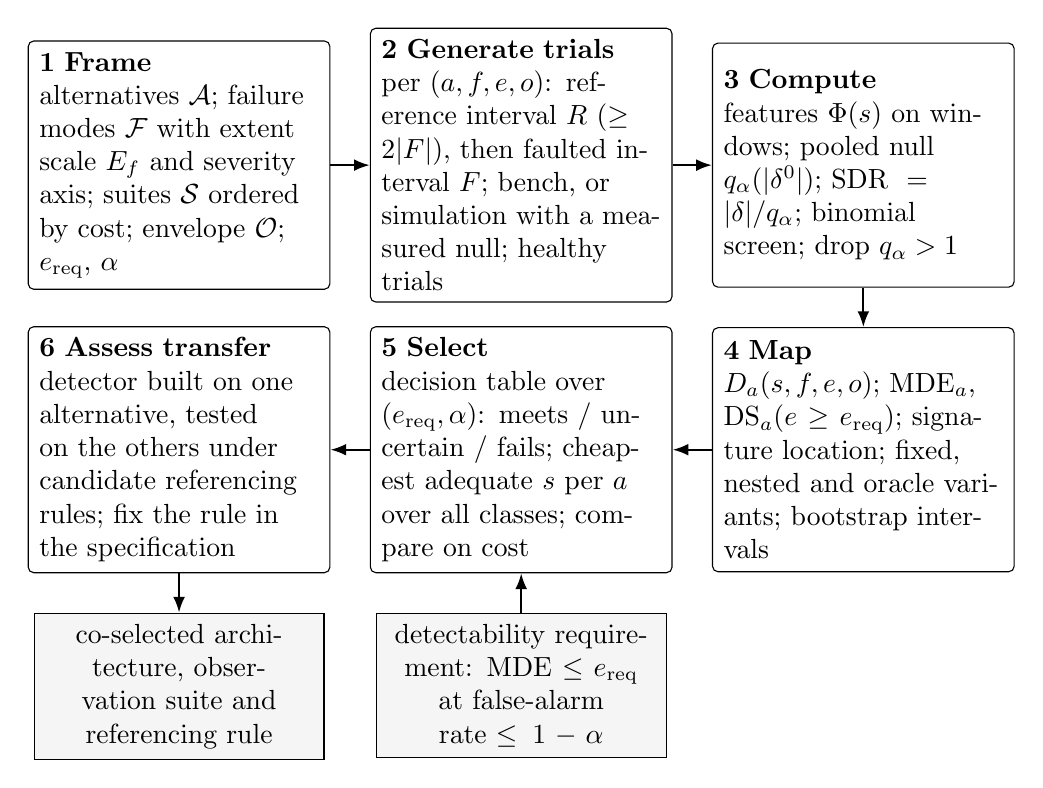
\begin{tikzpicture}[
  font=\normalsize,
  box/.style={draw, rounded corners=2pt, align=left, inner sep=4pt, text width=3.55cm, minimum height=3.1cm},
  data/.style={draw, align=center, inner sep=4pt, text width=3.4cm, fill=black!4},
  arr/.style={-{Latex[length=2mm]}, thick},
  node distance=5mm and 5mm
]
\node[box] (s1) {\textbf{1 Frame}\\ alternatives $\mathcal{A}$; failure modes $\mathcal{F}$ with extent scale $E_f$ and severity axis; suites $\mathcal{S}$ ordered by cost; envelope $\mathcal{O}$; $e_{\mathrm{req}}$, $\alpha$};
\node[box, right=of s1] (s2) {\textbf{2 Generate trials}\\ per $(a,f,e,o)$: reference interval $R\ (\ge 2|F|)$, then faulted interval $F$; bench, or simulation with a measured null; healthy trials};
\node[box, right=of s2] (s3) {\textbf{3 Compute}\\ features $\Phi(s)$ on windows; pooled null $q_\alpha(|\delta^0|)$; $\mathrm{SDR}=|\delta|/q_\alpha$; binomial screen; drop $q_\alpha>1$};
\node[box, below=of s3] (s4) {\textbf{4 Map}\\ $D_a(s,f,e,o)$; $\mathrm{MDE}_a$, $\mathrm{DS}_a(e\ge e_{\mathrm{req}})$; signature location; fixed, nested and oracle variants; bootstrap intervals};
\node[box, left=of s4] (s5) {\textbf{5 Select}\\ decision table over $(e_{\mathrm{req}},\alpha)$: meets / uncertain / fails; cheapest adequate $s$ per $a$ over all classes; compare on cost};
\node[box, left=of s5] (s6) {\textbf{6 Assess transfer}\\ detector built on one alternative, tested on the others under candidate referencing rules; fix the rule in the specification};
\draw[arr] (s1) -- (s2);
\draw[arr] (s2) -- (s3);
\draw[arr] (s3) -- (s4);
\draw[arr] (s4) -- (s5);
\draw[arr] (s5) -- (s6);
\node[data, below=5mm of s6] (out) {co-selected architecture, observation suite and referencing rule};
\draw[arr] (s6) -- (out);
\node[data, below=5mm of s5] (req) {detectability requirement: $\mathrm{MDE}\le e_{\mathrm{req}}$ at false-alarm rate $\le 1-\alpha$};
\draw[arr] (req) -- (s5);
\end{tikzpicture}
\caption{The six-step design procedure; steps 3--4 are fixed by Eqs.~(\ref{eq:delta})--(\ref{eq:sdr}), steps 1, 2, 5 and 6 follow the default rules of Section~\ref{sec:procedure}}\label{fig:method}
\end{figure}

The procedure (Fig.~\ref{fig:method}) has six steps. Steps 3--4 are mechanical and fully specified by Eqs.~(\ref{eq:delta})--(\ref{eq:sdr}); steps 1, 2, 5 and 6 are design decisions, for which the method supplies default rules.
\begin{enumerate}
  \item \textbf{Frame.} Enumerate $\mathcal{A}$, the classes $\mathcal{F}$ with an extent scale $E_f$ realisable in every alternative and a physical severity axis, the suites $\mathcal{S}$ and the envelope $\mathcal{O}$. Set $e_{\mathrm{req}}$ as the smallest extent whose growth to an unacceptable consequence is faster than the inspection interval, and $1-\alpha$ as the per-trial false-alarm rate the operator tolerates over that interval. Order the suites by cost: an ordinal rank by added hardware and integration by default, a monetary cost including installation and maintenance when available.
  \item \textbf{Generate trials.} For each $(a,f,e,o)$ obtain trials with a healthy reference interval of at least twice the faulted duration, immediately followed by the faulted interval; test at least the extent levels that bracket $e_{\mathrm{req}}$ and the corners of the envelope; include enough healthy trials with the same timing for the screen (nine allow the binomial rule above). At the test stage these are prototype or benchmark experiments; at the design stage the faulted numerator is simulated and the null is supplied as in Section~\ref{sec:design-stage}.
  \item \textbf{Compute.} Extract $\Phi(s)$ for all suites on sliding windows within the intervals, form the pooled null per alternative and feature, compute the SDR per trial, apply the screen.
  \item \textbf{Map.} Build $D_a(s,f,e,o)$ and summarise it into $\mathrm{MDE}_a$, $\mathrm{DS}_a$ and the signature location for the fixed, nested and oracle variants, with bootstrap intervals.
  \item \textbf{Select.} Build the decision table: for each alternative, class and suite and for the candidate values of $e_{\mathrm{req}}$ and $\alpha$, classify the suite as \emph{meets} when the bootstrap probability that $\mathrm{MDE}\le e_{\mathrm{req}}$ is at least 0.95, \emph{fails} when it is at most 0.05, and \emph{uncertain} otherwise. The adequate suite of an alternative is the cheapest that meets the requirement for \emph{every} class; an uncertain verdict is resolved by more trials around $e_{\mathrm{req}}$ or by specifying the next suite as a fallback. The alternatives are then compared on the cost of their adequate suites together with the other selection criteria; the architecture decision is affected only when, for some alternative, no affordable suite meets the requirement, otherwise the method changes the monitoring specification and says so.
  \item \textbf{Assess transfer.} If the suite and its detector must serve a family of alternatives, test whether a detector built on one alternative's trials detects the others' faults under the candidate feature-referencing rules (physical units; scaled on the target's healthy trials; referenced to each trial's own preceding healthy interval). The rule that transfers becomes part of the monitoring specification.
\end{enumerate}

\subsection{Design-stage instantiation}\label{sec:design-stage}

The demonstration in this paper is a test-stage instantiation on built machines. A design-stage instantiation must supply the two ingredients of the SDR separately. The numerator---the change of a feature under a fault of extent $e$---is what a finite-element or circuit model of each alternative with the fault injected can provide \citep{Vaseghi2009}. The denominator---the healthy non-stationarity of sensor noise, controller activity, thermal drift and operating-point wander---is a property of hardware and environment that such a model does not reproduce, and a simulated SDR that supplied its own null would be optimistic by an unknown factor. The null must therefore come from measured healthy records of hardware of the same class (a predecessor product, a prototype of one alternative, or a benchmark such as the one used here), transferred to the other alternatives on the assumption that the healthy non-stationarity of a feature depends on the sensing and control chain more than on the machine; the assumption is testable by comparing the null quantiles of the alternatives for which hardware exists (Table~\ref{tab:decomp} does so for the two machines on one bench), and a simulated instantiation is validated by comparing simulated and measured SDR on a few physical trials, the role the three benches would play in a design study of the next generator.

\subsection{Scope}\label{sec:scope}

The method applies to failure-mode classes that can be seeded at a known extent, at a stationary operating point, with a healthy interval immediately before the fault, in every alternative; the extent scale must be realisable in all of them, and the physical severity axis is declared beside it. It evaluates detectability by a threshold on interval means, not the time to detection, and stops at detection: isolation, severity estimation and remaining-life prediction presuppose detectability and can be built on the same trials. It does not model the cost of missed detection, which enters through $e_{\mathrm{req}}$ and $\alpha$. Run-to-failure data, in which the fault grows gradually and no healthy interval precedes a known onset, do not fit the trial structure and would need a different null.
%% ----------------------------------------------------------------------
%% demo
%% ----------------------------------------------------------------------

\section{Demonstration on three wind-turbine generators}\label{sec:demo}

\subsection{Alternatives and data}\label{sec:data}

The three alternatives are laboratory-scale generators of the same power class on instrumented test benches at the University of S\~ao Paulo, published as open benchmark datasets (Table~\ref{tab:alternatives}, Fig.~\ref{fig:alternatives}). The PMSG \citep{Tominaga2025pmsg} and the SCIG \citep{Tominaga2025scig} are four-pole, 230\,V, double-star machines from the same manufacturer, rated 2.5\,kVA and 2.5\,kW, installed on the \emph{same} bench: the same induction-motor prime mover and frequency converter, the same rapid-control-prototyping platform and field-oriented control (FOC; rotor angle from an encoder for the PMSG, from a flux observer for the SCIG), the same sensors, acquisition (20\,kHz, 3\,s records), fault-insertion hardware and test script. The variable-speed WFSG \citep{Tominaga2024gen} is a 2\,kVA four-salient-pole machine on an earlier bench of the same group \citep{Rocha2023} with a three-level converter, FOC with encoder angle, 4\,kHz acquisition and 1.3\,s records. The PMSG--SCIG pair is therefore a controlled comparison in which everything but the machine and the control structure it requires is held fixed; the WFSG is a third alternative with the same fault protocol on a different bench, analysed with that difference kept explicit. Terminal voltages are measured by each bench's voltage transducers, whose bandwidth the data papers do not document, so the terminal-voltage features carry the sensing chain of their bench as well as the machine.

\begin{table}[t]
\tabsize
\setlength{\tabcolsep}{4pt}
\caption{The three alternatives; the PMSG and SCIG share one bench and one protocol, the WFSG bench differs where indicated}\label{tab:alternatives}
\begin{tabular}{@{}p{2.4cm}p{2.8cm}p{3.3cm}p{3.4cm}@{}}
\toprule
 & PMSG & SCIG & WFSG (variable speed) \\
\midrule
Rating, poles & 2.5\,kVA, 4 & 2.5\,kW, 4 & 2\,kVA, 4 salient \\
Excitation & permanent magnets & induction (magnetising current) & wound field, static exciter \\
Converter and control & 2L, FOC with encoder & 2L, FOC with flux observer & 3L-NPC, FOC with encoder \\
Acquisition & 20\,kHz, 3\,s & 20\,kHz, 3\,s & 4\,kHz, 1.3\,s \\
Reference / faulted interval & 0.68\,s / 0.36\,s & 0.68\,s / 0.36\,s & 0.49\,s / 0.06--0.28\,s \\
Fault impedance & 2.6\,$\Omega$ & 2.6\,$\Omega$ & 1, 2.83, 5.66, 11.32\,$\Omega$ \\
Operating points & 3 speeds $\times$ 3 torques & same & 716--1910\,rpm, 4 torque levels (sparse) \\
Healthy trials & 9 & 9 & none \\
Fault trials & 216 & 216 & 438 (198 at 2.83\,$\Omega$) \\
\botrule
\end{tabular}
\footnotetext{Ratings as given by the manufacturer (kVA for the synchronous machines, kW for the induction machine). 2L: two-level converter; 3L-NPC: three-level neutral-point-clamped converter; FOC: field-oriented control.}
\end{table}

%% ----------------------------------------------------------------------
%% fig_alternatives
%% ----------------------------------------------------------------------

\begin{figure}[t]
\centering
\definecolor{pmsgc}{HTML}{2A78D6}
\definecolor{scigc}{HTML}{EB6834}
\definecolor{wfsgc}{HTML}{1BAF7A}
\begin{tikzpicture}[
  font=\normalsize, x=1cm, y=1cm, line cap=round, line join=round,
  frame/.style={draw=black!70, line width=0.8pt},
  hd/.style={anchor=south, inner sep=1pt},
  sub/.style={anchor=north, inner sep=1pt, text width=12.6cm, align=center}
]
%% One row per alternative: turbine rotor, shaft, generator (stator ring with the rotor symbol),
%% three-phase stator connection, back-to-back converter (ac/dc, dc link, dc/ac) and grid.
\newcommand{\chain}[1]{%
  \foreach \ang in {90,210,330} {
    \begin{scope}[shift={(1.1,#1)}, rotate=\ang-90]
      \path[frame, fill=black!15] (0.07,0) .. controls (0.18,0.22) and (0.13,0.52) .. (0,0.7)
                                   .. controls (-0.13,0.52) and (-0.18,0.22) .. (-0.07,0) -- cycle;
    \end{scope}
  }
  \fill[black!70] (1.1,#1) circle (0.09);
  \draw[black!55, line width=2.2pt] (1.25,#1) -- (3.7,#1);
  \filldraw[frame, fill=black!8] (4.3,#1) circle (0.62);
  \filldraw[frame, fill=white] (4.3,#1) circle (0.5);
  \draw[frame] (4.92,#1) -- (7.2,#1);
  \foreach \s in {-0.09,0,0.09} { \draw[frame] (6.0+\s,#1-0.12) -- (6.14+\s,#1+0.12); }
  \filldraw[frame, fill=black!5] (7.2,#1-0.4) rectangle (8.0,#1+0.4);
  \draw[frame] (7.2,#1-0.4) -- (8.0,#1+0.4);
  \node[inner sep=0] at (7.41,#1+0.2) {$\sim$};
  \node[inner sep=0] at (7.79,#1-0.2) {$=$};
  \draw[frame] (8.0,#1+0.1) -- (8.3,#1+0.1);
  \draw[frame] (8.0,#1-0.1) -- (8.3,#1-0.1);
  \filldraw[frame, fill=black!5] (8.3,#1-0.4) rectangle (9.1,#1+0.4);
  \draw[frame] (8.3,#1-0.4) -- (9.1,#1+0.4);
  \node[inner sep=0] at (8.51,#1+0.2) {$=$};
  \node[inner sep=0] at (8.89,#1-0.2) {$\sim$};
  \draw[frame] (9.1,#1) -- (11.3,#1);
  \draw[black!70, line width=2.4pt] (11.3,#1-0.5) -- (11.3,#1+0.5);
}
%% column headers
\node[hd] at (1.1,0.85) {turbine rotor};
\node[hd] at (4.3,0.85) {generator};
\node[hd] at (8.15,0.85) {converter};
\node[hd] at (11.3,0.85) {grid};
%% (a) SCIG: squirrel cage
\chain{0}
\draw[scigc, line width=1.1pt] (4.3,0) circle (0.42);
\draw[scigc, line width=1.1pt] (4.3,0) circle (0.26);
\foreach \a in {0,30,...,330} { \draw[scigc, line width=1.1pt] (4.3,0) ++(\a:0.26) -- ++(\a:0.16); }
\node[sub] at (6.2,-0.8) {(a) SCIG};
%% (b) WFSG: field winding on the rotor
\chain{-2.1}
\draw[black!50, line width=0.6pt] (4.3,-2.1) circle (0.42);
\draw[wfsgc, line width=1.1pt, decorate, decoration={coil, aspect=0.6, segment length=1.9mm, amplitude=1.9mm}] (3.9,-2.1) -- (4.7,-2.1);
\node[sub] at (6.2,-2.9) {(b) WFSG};
%% (c) PMSG: permanent magnets on the rotor surface
\chain{-4.2}
\draw[black!50, line width=0.6pt] (4.3,-4.2) circle (0.31);
\foreach \a in {0,120,240} { \draw[pmsgc, line width=2.8pt] (4.3,-4.2) ++(\a+7:0.4) arc[start angle=\a+7, end angle=\a+53, radius=0.4]; }
\foreach \a in {60,180,300} { \draw[black!40, line width=2.8pt] (4.3,-4.2) ++(\a+7:0.4) arc[start angle=\a+7, end angle=\a+53, radius=0.4]; }
\node[sub] at (6.2,-5.0) {(c) PMSG};
\end{tikzpicture}
\caption{The three alternatives as generator systems: turbine rotor, generator with its rotor excitation (squirrel cage, field winding, permanent magnets), back-to-back converter and grid}\label{fig:alternatives}
\end{figure}

\subsection{Failure-mode class and extent scale}\label{sec:extent}

All three machines were built with 24 tapped derivation points along their stator windings at the same relative positions, so that a short-circuit between two taps realises a fault of known extent; the tap positions are identical in the three data papers, which is what makes the extent scale realisable in every alternative. Two classes are used (Fig.~\ref{fig:faults}): inter-turn short-circuits (both taps on the same branch) and inter-winding short-circuits (taps on the two parallel branches of a phase). The extent $e$ is the fraction of a branch between the two taps; it ranges from 2.7\,\% to 12.1\,\% for the twelve inter-turn cases and from 2.3\,\% to 40.2\,\% for the twelve inter-winding cases. Extents that coincide at different winding locations (2.8\,\% twice, 7.4\,\% three times, 11.6\,\% twice) form one extent level. Faults were closed through a contactor and a series resistance after the machine had reached steady state: 2.6\,$\Omega$ for 0.4\,s on the PMSG and SCIG; on the WFSG the experimenters raised the resistance with extent (1\,$\Omega$ for the inter-turn cases below 11\,\%, 2.83\,$\Omega$ for the remaining inter-turn cases and the small inter-winding cases, 5.66 and 11.32\,$\Omega$ for the large inter-winding cases), so that on that bench extent and impedance are confounded. The fault current is measured on all benches; it is used only as ground truth for the physical severity axis, never as a feature. Because the series resistance is of the order of the winding impedance of these small machines, the fault current is essentially the voltage induced in the shorted turns divided by the resistance: a \emph{resistor-limited} severity, unlike a bolted fault, which the leakage reactance of the shorted turns limits (Section~\ref{sec:res-severity}).

%% ----------------------------------------------------------------------
%% fig_faults
%% ----------------------------------------------------------------------

\begin{figure}[t]
\centering
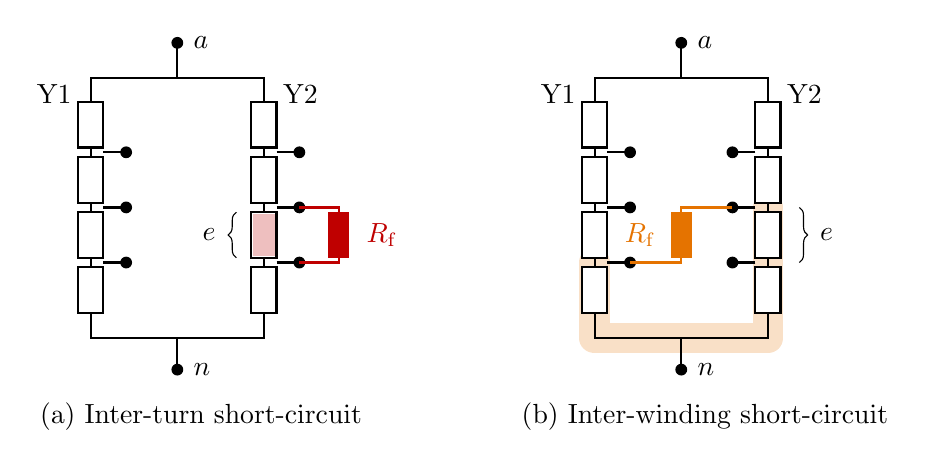
\begin{tikzpicture}[
  font=\normalsize, x=1cm, y=1cm,
  wire/.style={thick},
  coil/.style={draw, thick, fill=white, minimum width=3.2mm, minimum height=5.8mm, inner sep=0},
  tap/.style={circle, fill=black, inner sep=0, minimum size=1.5mm},
  rf/.style={draw, thick, fill=white, minimum width=2.4mm, minimum height=5.5mm, inner sep=0},
  it/.style={red!75!black},
  iw/.style={orange!90!black}
]
%% One phase (a--n) of the double-star stator: two parallel branches Y1 and Y2 of four coil groups with
%% tapped derivation points. Panel (a) inter-turn fault, panel (b) inter-winding fault.
\foreach \dx in {0, 6.4} {
  % circulating path of the inter-winding fault (panel b only), drawn first so that it lies behind
  \ifdim \dx pt > 1pt
    \draw[iw, line width=11pt, line cap=round, line join=round, opacity=0.22]
      (\dx+0.9,1.71) -- (\dx+0.9,0.75) -- (\dx+3.1,0.75) -- (\dx+3.1,2.41);
  \fi
  % terminal, junctions, branches, neutral
  \node[tap, label={right:$a$}] at (\dx+2.0,4.5) {};
  \draw[wire] (\dx+2.0,4.5) -- (\dx+2.0,4.05) -- (\dx+0.9,4.05) -- (\dx+0.9,0.75) -- (\dx+2.0,0.75) -- (\dx+2.0,0.35);
  \draw[wire] (\dx+2.0,4.05) -- (\dx+3.1,4.05) -- (\dx+3.1,0.75) -- (\dx+2.0,0.75);
  \node[tap, label={right:$n$}] at (\dx+2.0,0.35) {};
  \node[anchor=east] at (\dx+0.78,3.85) {Y1};
  \node[anchor=west] at (\dx+3.22,3.85) {Y2};
  \foreach \bx in {0.9, 3.1} {
    \foreach \cy in {3.46, 2.76, 2.06, 1.36} { \node[coil] at (\dx+\bx,\cy) {}; }
  }
  % taps of Y1 point into the gap between the branches
  \foreach \ty in {3.11, 2.41, 1.71} {
    \draw[wire] (\dx+1.06,\ty) -- (\dx+1.35,\ty); \node[tap] at (\dx+1.35,\ty) {};
  }
}
%% (a) inter-turn: two taps of one branch (Y2) shorted through R_f; the shorted coil group is shaded
\begin{scope}
  \foreach \ty in {3.11, 2.41, 1.71} {
    \draw[wire] (3.26,\ty) -- (3.55,\ty); \node[tap] at (3.55,\ty) {};
  }
  \fill[it, opacity=0.25] (2.96,2.33) rectangle (3.24,1.79);
  \draw[it, thick] (3.55,2.41) -- (4.05,2.41) -- (4.05,1.71) -- (3.55,1.71);
  \node[rf, it] at (4.05,2.06) {};
  \node[it, anchor=west] at (4.28,2.06) {$R_{\mathrm{f}}$};
  \draw[decorate, decoration={brace, amplitude=3pt}] (2.75,1.77) -- (2.75,2.35) node[midway, left=4pt] {$e$};
  \node at (2.3,-0.25) {(a) Inter-turn short-circuit};
\end{scope}
%% (b) inter-winding: a tap of Y1 and a tap of Y2 at different positions shorted through R_f;
%% the fault current circulates through the lower parts of both branches and the neutral link
\begin{scope}[shift={(6.4,0)}]
  \foreach \ty in {3.11, 2.41, 1.71} {
    \draw[wire] (2.94,\ty) -- (2.65,\ty); \node[tap] at (2.65,\ty) {};
  }
  \draw[iw, thick] (1.35,1.71) -- (2.0,1.71) -- (2.0,2.41) -- (2.65,2.41);
  \node[rf, iw] at (2.0,2.06) {};
  \node[iw, anchor=east] at (1.8,2.06) {$R_{\mathrm{f}}$};
  \draw[decorate, decoration={brace, mirror, amplitude=3pt}] (3.5,1.71) -- (3.5,2.41) node[midway, right=4pt] {$e$};
  \node at (2.3,-0.25) {(b) Inter-winding short-circuit};
\end{scope}
\end{tikzpicture}
\caption{Inter-turn (\textbf{a}) and inter-winding (\textbf{b}) short-circuits through $R_{\mathrm{f}}$ between taps of one phase of the double-star stator (schematic); $e$ is the fraction of a branch between the taps}\label{fig:faults}
\end{figure}

The PMSG and SCIG matrix is complete: 24 fault cases $\times$ 3 speeds (1200, 1500, 1800\,rpm) $\times$ 3 torques (5.2, 6.4, 8.0\,N\,m), the torque--speed pairs scaled from the operating region of the International Energy Agency (IEA) 15\,MW reference turbine \citep{Gaertner2020} to the laboratory speed range (the electrical frequency is not scaled), plus the healthy condition at each operating point; the SCIG generates with slip, at 59.6\,Hz at 1800\,rpm. The WFSG matrix covers the same 24 tap pairs at six speeds (716--1910\,rpm) and four per-unit torque levels, sparsely and with two to six repetitions, so its operating points are not matched to the other two. The WFSG benchmark also contains phase-to-phase faults, a class absent from the PMSG/SCIG protocol; they are excluded from every analysis. The analyses use the WFSG's 438 inter-turn and inter-winding trials at all impedances for the null, the feature ranking and the detectable shares, with the impedance as a covariate, and the 198 trials at 2.83\,$\Omega$---the impedance closest to the PMSG/SCIG value, covering four inter-turn tap pairs of 11.6--12.1\,\% and four inter-winding pairs of 2.3--10.6\,\%---for the minimum detectable extent and the decision table.

\subsection{Observation suites and features}\label{sec:suites}

Five observation suites are considered, ordered by the data access, hardware and integration they add to a bare generator--converter set (Table~\ref{tab:suitedef}). \emph{Drive-internal} uses only quantities the converter controller already has; \emph{3\,CT} (three current transducers) uses the three phase currents---from dedicated transducers or from the converter's own current sensors routed to a monitoring system---with angle-free features, so that for a converter-fed machine its cost is data access and bandwidth rather than hardware; \emph{3\,CT + 3\,VT} adds three terminal voltage transducers (VT); \emph{3\,CT + 3\,VT + drive} adds controller access, which also allows the measured terminal voltages to be transformed into the synchronous frame; and \emph{+ torque transducer} adds a shaft torque sensor. For the WFSG the field current is an additional drive-internal observable (the \emph{excitation} suite), available because its exciter is static \citep{Neti2009}. Each feature is assigned to the cheapest suite whose measurements suffice to compute it. The suites are those the datasets can populate (zero-sequence voltage, stray flux, winding temperature, vibration and partial discharge are not recorded, and the angle-free Park's-vector features were not computed), so the suite conclusions hold among the suites and features considered; the zero-sequence current is not used because the star points are isolated.

\begin{table}[t]
\tabsize
\setlength{\tabcolsep}{4pt}
\caption{Observation suites and the features they can compute}\label{tab:suitedef}
\begin{tabular}{@{}p{2.3cm}p{3.0cm}p{7.0cm}@{}}
\toprule
Suite & Added access / hardware & Features \\
\midrule
Drive-internal & controller data & $I_d, I_q$: std, 1$f_e$, 2$f_e$; $V_d^{\mathrm{cmd}}, V_q^{\mathrm{cmd}}$: 2$f_e$; PI outputs $d,q$: std, 2$f_e$; duty-cycle negative sequence $D_2/D_1$; $T_e$: std, 1$f_e$, 2$f_e$; DC-link std; speed std \\
3\,CT & three phase currents, no angle & $I_2/I_1$, RMS unbalance, harmonics 3, 5, 7 of $I_a$ relative to the fundamental, THD \\
3\,CT + 3\,VT & + 3 voltage transducers & 3\,CT features + $V_2/V_1$ \\
3\,CT + 3\,VT + drive & + controller data & all of the above + measured $V_d, V_q$: 2$f_e$ \\
+ torque transducer & + shaft torque sensor & + $T_m$: std, 1$f_e$, 2$f_e$ \\
Excitation (WFSG) & field-current measurement & $I_f$: std, 2$f_e$ \\
\botrule
\end{tabular}
\footnotetext{$f_e$: electrical frequency; 1$f_e$, 2$f_e$: amplitude of the component at once and twice the electrical frequency; $I_1, I_2$ ($V_1, V_2$): positive- and negative-sequence magnitudes at $f_e$; std: standard deviation; THD: total harmonic distortion; PI: proportional--integral.}
\end{table}

Features are computed on sliding windows of $n_c$ electrical cycles with a hop of one cycle; the electrical frequency and the phase rotation are estimated per window from the current space vector, so that the external suites need no angle sensor. Appendix~\ref{app:features} defines every feature and states which WFSG channels are measured and which commanded.

\subsection{Computation}\label{sec:computation}

For the PMSG and SCIG the reference interval is the 0.68\,s before the contactor command, split into $R_1$ (0.32\,s) and $R_2$ (0.36\,s), and the faulted interval runs from 30\,ms after the command to 10\,ms before its release; for the WFSG the fault interval is located from the measured fault current and the reference interval (0.49\,s) is split at 0.30\,s. Appendix~\ref{app:computation} lists all interval boundaries, thresholds, seeds and model settings. The main PMSG--SCIG comparison uses $n_c=5$; the three-alternative comparison uses $n_c=3$ for all three machines because the WFSG fault intervals are short. The sensitivity of every conclusion to $n_c\in\{3,5,8\}$ and to $\alpha\in\{0.90,0.95,0.99\}$ is reported, with the screen applied at each setting. The null is pooled over all 225 records of each of the PMSG and SCIG and over the 438 WFSG records, every record contributing a healthy reference interval. Uncertainty is quantified by bootstrap with 2000 resamples: the median SDR and the detectable share of a class are resampled over the twelve tap pairs, the same pairs for both machines so that the SCIG/PMSG ratio is matched; the minimum detectable extent is resampled over the operating-point trials within each extent level; shares also carry Wilson intervals; the null quantile is held at its full-sample value. The decision table uses 1000 resamples per suite, alternative, class and $\alpha$, with $e_{\mathrm{req}}\in\{3,5,8,12\}$\,\%.

Step 6 of the procedure is instantiated as a window-level change detector: a gradient-boosted decision-tree (GBDT) classifier \citep{Friedman2001} and, for the PMSG--SCIG pair, a logistic regression, trained to separate faulted windows from healthy ones. Within an alternative the detector is evaluated by five-fold cross-validation grouped by tap pair (healthy trials grouped by speed), so that the tested fault locations are never seen in training; across alternatives it is trained on all trials of one machine and tested on all trials of another. Three feature-referencing rules are compared: physical units; features $z$-scored on the target machine's healthy trials (a commissioning baseline); and the absolute $z$-score of each window against the \emph{first half} of its own trial's reference interval. Negatives are the reference and recovery windows of all trials plus the fault-interval windows of the healthy trials, the only negatives that contain the contactor operation without a fault. Because the windows used to normalise a trial are trivially separable under the third rule, every metric is also reported on the out-of-reference windows, and the false-alarm rate of the threshold that gives 1\,\% false positives on all negatives is reported on the healthy trials' fault-time windows; the true-positive rate at 1\,\% false-positive rate is a point of the receiver operating characteristic, not an operating threshold.

All computations are implemented in Python and released with the paper; the pipeline runs from the feature caches to every table and figure in under thirty minutes on a four-core machine. A large language model assisted in writing the analysis code and in drafting and editing the text; every analysis and reference was verified by the author (see the declarations).
%% ----------------------------------------------------------------------
%% results
%% ----------------------------------------------------------------------

\section{Results}\label{sec:results}

\subsection{The same design-level fault is not the same physical fault}\label{sec:res-severity}

For the same tap pair the SCIG's fault current is about 10\,\% lower than the PMSG's (medians 3.3 against 3.7\,A for inter-turn and 7.7 against 8.5\,A for inter-winding pairs), but the difference that matters for detection is relative to what the stator sensors see: the fault current is 1.45 times the pre-fault stator current (RMS to RMS, median over pairs) in the PMSG and 0.63 times in the SCIG for inter-turn faults, and 3.3 against 1.5 times for inter-winding faults, because the SCIG's stator current carries the magnetising component (5.3 against 2.6\,A RMS before the fault). The WFSG trials at the matching impedance give 1.20 (inter-turn, 11.6--12.1\,\%) and 1.03 (inter-winding, 2.3--10.6\,\%), and 0.65 at the lower impedance used for its small inter-turn extents. Being resistor-limited (Section~\ref{sec:extent}), these currents scale with volts per turn and speed; a bolted fault would reach several times rated current and---the first-order difference between the topologies---could be de-excited in the SCIG and the WFSG but not in the PMSG. A fault specified as ``$e$\,\% of a winding'' therefore arrives at the sensors of the three alternatives as three different physical events; Section~\ref{sec:res-mde} uses both axes.

\subsection{Where the signature appears, and why the SDR differs}\label{sec:res-where}

The null of the SDR differs by up to a factor of 35 between the PMSG and the SCIG (Table~\ref{tab:decomp}, columns $q_{95}$), and not only in sensed quantities: the null of the duty-cycle negative sequence, a controller output that involves no sensor, is nine times larger on the PMSG, so the healthy non-stationarity is a property of the machine--drive combination, not of the transducers alone. The table also decomposes the SCIG/PMSG ratio of median SDR: for inter-turn faults the PMSG's relative changes are the \emph{larger} ones on every feature (SCIG/PMSG ratio of median $|\delta|$ 0.37--0.71), and the SCIG's higher SDR is entirely a quieter null (ratio of null quantiles 2.6--35); for inter-winding faults the numerators are comparable (0.3--1.4) and the denominators again decide.

%% BEGIN GENERATED tab_decomp -- written by scripts/make_tables.py from results/tables; do not edit by hand
\begin{table}[t]
\tabsize
\setlength{\tabcolsep}{3pt}
\caption{SCIG/PMSG ratio of median SDR decomposed into numerator and denominator, five-cycle windows}\label{tab:decomp}
\begin{tabular}{@{}llccccccc@{}}
\toprule
Class & Feature & $|\delta|$ P & $|\delta|$ S & $q_{95}$ P & $q_{95}$ S & Num. & Den. & SDR ratio \\
\midrule
inter-turn & $V_2/V_1$ & 0.257 & 0.136 & 0.086 & 0.033 & 0.53 & 2.64 & 1.40 \\
inter-turn & $I_2/I_1$ & 0.238 & 0.152 & 0.162 & 0.034 & 0.64 & 4.82 & 3.08 \\
inter-turn & $I_d$\,2$f_e$ & 0.291 & 0.107 & 0.563 & 0.016 & 0.37 & 35.09 & 12.95 \\
inter-turn & PI$_d$\,2$f_e$ & 0.289 & 0.107 & 0.557 & 0.016 & 0.37 & 34.71 & 12.91 \\
inter-turn & $V_q$\,2$f_e$ & 0.222 & 0.155 & 0.165 & 0.060 & 0.70 & 2.73 & 1.91 \\
inter-turn & $V_q^{\mathrm{cmd}}$\,2$f_e$ & 0.197 & 0.139 & 0.162 & 0.039 & 0.71 & 4.17 & 2.94 \\
inter-turn & $D_2/D_1$ & 0.251 & 0.111 & 0.090 & 0.010 & 0.44 & 8.96 & 3.98 \\
inter-winding & $V_2/V_1$ & 5.318 & 1.569 & 0.086 & 0.033 & 0.30 & 2.64 & 0.78 \\
inter-winding & $I_2/I_1$ & 1.833 & 1.869 & 0.162 & 0.034 & 1.02 & 4.82 & 4.91 \\
inter-winding & $I_d$\,2$f_e$ & 2.335 & 1.188 & 0.563 & 0.016 & 0.51 & 35.09 & 17.85 \\
inter-winding & PI$_d$\,2$f_e$ & 2.344 & 1.188 & 0.557 & 0.016 & 0.51 & 34.71 & 17.60 \\
inter-winding & $V_q$\,2$f_e$ & 3.688 & 1.495 & 0.165 & 0.060 & 0.41 & 2.73 & 1.11 \\
inter-winding & $V_q^{\mathrm{cmd}}$\,2$f_e$ & 0.845 & 1.184 & 0.162 & 0.039 & 1.40 & 4.17 & 5.84 \\
inter-winding & $D_2/D_1$ & 2.942 & 0.854 & 0.090 & 0.010 & 0.29 & 8.96 & 2.60 \\
\botrule
\end{tabular}
\footnotetext{Num.: SCIG/PMSG ratio of the median relative change under fault $|\delta|$; Den.: ratio of null quantiles $q_{95}^{\mathrm{PMSG}}/q_{95}^{\mathrm{SCIG}}$; P: PMSG; S: SCIG.}
\end{table}
%% END GENERATED tab_decomp

Fig.~\ref{fig:features} shows the median SDR of every feature for the three alternatives (the WFSG pooled over its fault impedances; features to the right of the dashed line at $\mathrm{SDR}=1$ are detectable in more than half of the trials). In the PMSG the terminal-voltage group carries the strongest signature in 67\,\% of inter-turn and 88\,\% of inter-winding trials, through $V_2/V_1$ (median SDR 3.0 and 62 at five-cycle windows; 76 and 94\,\% of trials detectable), and the stator-current negative sequence $I_2/I_1$ is weak for inter-turn faults (median SDR 1.5, 56\,\%). In the SCIG the controller group is strongest in 56 and 67\,\% of trials, through the 2$f_e$ ripple of the $d$-axis current and its PI output (6.7 and 74; 79 and 100\,\%), the stator-current group in 28--33\,\% and the terminal-voltage group in 13\,\% and none. The two machines rank the 30 common features with a Spearman correlation of 0.70 (inter-turn) and 0.89 (inter-winding): the same features are informative in both, in a different order. In the WFSG the strongest inter-turn features are $V_2/V_1$, the $q$-axis current ripple and the commanded $q$-axis voltage, and for inter-winding faults the $q$-axis ripple, the commanded voltage, the duty cycles and the third current harmonic; its field-current 2$f_e$ ripple, an observable the other two machines lack, detected 86\,\% of the inter-turn trials at the matching impedance and all inter-winding trials (Table~\ref{tab:suites3}). The physical quantity behind the relocation is the incremental negative-sequence impedance $\Delta V_2/\Delta I_2$ seen at the terminals under inter-winding faults: 15 [11, 18]\,$\Omega$ in the PMSG, 7.0 [6.6, 7.5]\,$\Omega$ in the SCIG and 11 [10, 13]\,$\Omega$ in the WFSG (medians and interquartile ranges over trials, three-cycle windows), i.e.\ the PMSG drive converts a given negative-sequence current disturbance into twice the terminal voltage that the SCIG drive does; for inter-turn faults the PMSG's negative-sequence current increments are of mixed sign with a median indistinguishable from zero, which is why current-side features see little there. Both machines run the same field-oriented controller but differ in angle source (encoder against flux observer), negative-sequence impedance and feature baselines (healthy medians of $I_2/I_1$, $V_2/V_1$ and $D_2/D_1$: 0.0055, 0.0009 and 0.0014 on the PMSG against 0.0079, 0.0020 and 0.0036 on the SCIG, and 0.0148, 0.0073 and 0.0039 on the WFSG), so the relocation belongs to the machine--drive combination, not to the control structure alone.

\begin{figure}[t]
\centering
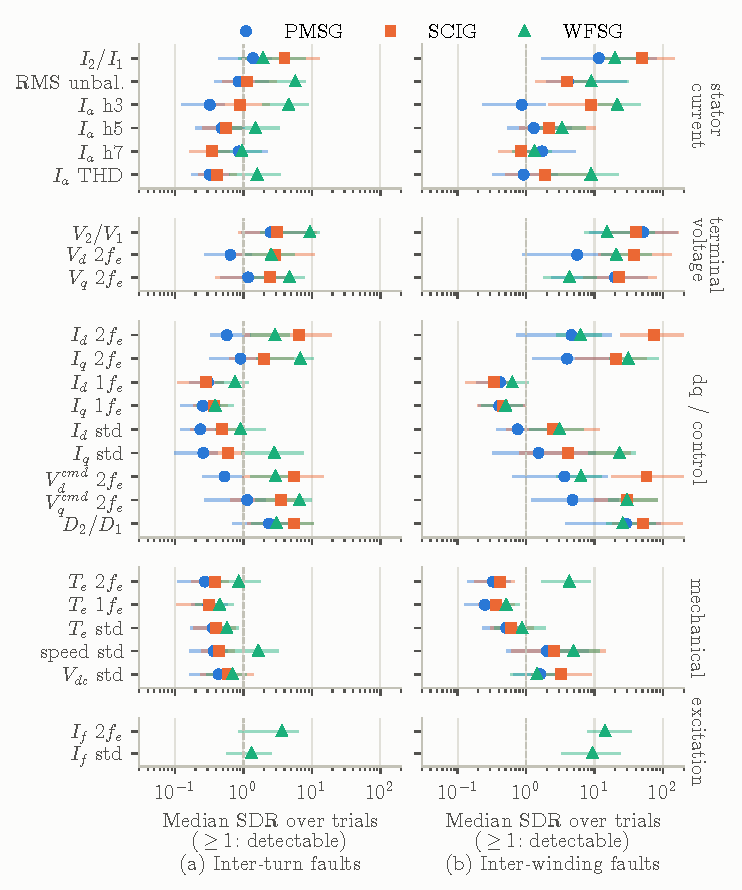
\includegraphics[width=\textwidth]{G_sdr_by_feature_3alt}
\caption{Median SDR of every feature (dot) with interquartile range (bar) for the three alternatives, three-cycle windows}\label{fig:features}
\end{figure}

\subsection{Minimum detectable extent}\label{sec:res-mde}

Table~\ref{tab:mde} gives the minimum detectable extent with its bootstrap interval, the detectable share with its Wilson interval and the median SDR with its tap-pair bootstrap interval for four representative features; Fig.~\ref{fig:severity} plots the SDR against the design-level extent (left; dots are trials, large markers the median per extent level, their shape the fault impedance) and against the physical severity axis (right; RMS fault current relative to the RMS pre-fault stator current, all trials). Through the terminal-voltage negative sequence the PMSG detects inter-turn faults from 3.8\,\% [2.8, 3.8] and the SCIG from 7.4\,\% [7.4, 7.4]; through the stator-current negative sequence both need 7.4\,\%, and through the $d$-axis ripple the PMSG needs 12.1\,\% and the SCIG 7.4\,\% [3.8, 7.4]. The smallest tested inter-turn level (2.7--2.8\,\%) is not reliably detectable on either machine by any single feature. For inter-winding faults the SCIG detects from the smallest tested extent (2.3\,\%) on every feature except the $q$-axis voltage ripple, while the PMSG needs 2.3\,\% [2.3, 14.3] on $V_2/V_1$ but 9.7\,\% on $I_2/I_1$ and 21.7\,\% on the $d$-axis ripple. The SDR rises with extent in every machine (Spearman 0.51--0.95), and the MDE intervals are wide because the tested extents form three clusters (about 3, 7.5 and 12\,\% for inter-turn faults), so the SCIG/PMSG ratio of median SDR is the better basis for comparison: 3.1 [1.3, 5.6] for $I_2/I_1$ and 12 [2.6, 30] for the $d$-axis ripple on inter-turn faults, but 1.1 [0.4, 4.6] for $V_2/V_1$ and 1.5 [0.5, 3.2] for the $q$-axis voltage ripple. The two machines differ where the signature relocates and are indistinguishable where it does not. On the physical axis (Fig.~\ref{fig:severity}, right) the picture is the same and independent of the tap-pair design: at equal fault-to-stator current ratio the SCIG's current-side features lie above the WFSG's, which lie above the PMSG's, while on $V_2/V_1$ the three machines nearly coincide. For the WFSG, whose small inter-turn extents were tested only at the lower impedance, the design-level MDE at the matching impedance is bounded by the smallest extent tested there (11.6\,\%, detectable in 78--98\,\% of trials depending on the suite); its 2.7--7.7\,\% inter-turn trials at 1\,$\Omega$ sit at SDR $\approx1$ on $V_2/V_1$ and $I_2/I_1$, and all its inter-winding extents from 2.3\,\% are detectable.

%% BEGIN GENERATED tab_mde -- written by scripts/make_tables.py from results/tables; do not edit by hand
\begin{table}[t]
\tabsize
\setlength{\tabcolsep}{2pt}
\caption{Minimum detectable extent, detectable share and median SDR with 95\,\% intervals for four features, PMSG and SCIG, five-cycle windows, $\alpha=0.95$}\label{tab:mde}
\begin{tabular}{@{}lllcccc@{}}
\toprule
Class & Feature & M. & MDE [CI] & DS [CI] & Median SDR [CI] & S/P ratio [CI] \\
\midrule
IT & $V_2/V_1$ & P & 3.8 [2.8, 3.8] & 76 [67, 83] & 2.99 [1.21, 12.5] & \\
 &  & S & 7.4 [7.4, 7.4] & 73 [64, 81] & 4.17 [0.949, 15.5] & 1.1 [0.378, 4.56] \\
IT & $I_2/I_1$ & P & 7.4 [7.4, 12.1] & 56 [47, 65] & 1.47 [0.601, 2.36] & \\
 &  & S & 7.4 [7.4, 7.4] & 75 [66, 82] & 4.52 [1.11, 11.7] & 3.07 [1.34, 5.63] \\
IT & PI$_d$\,2$f_e$ & P & 12.1 [11.6, 12.1] & 31 [23, 40] & 0.518 [0.389, 1.11] & \\
 &  & S & 7.4 [3.8, 7.4] & 78 [69, 85] & 6.69 [1.3, 18.3] & 11.8 [2.59, 28.8] \\
IT & $V_q$\,2$f_e$ & P & 7.4 [7.4, 11.6] & 57 [48, 66] & 1.35 [0.791, 4.58] & \\
 &  & S & 7.4 [7.4, 7.7] & 60 [51, 69] & 2.58 [0.516, 5.33] & 1.49 [0.464, 3.21] \\
IW & $V_2/V_1$ & P & 2.3 [2.3, 14.3] & 94 [88, 97] & 61.9 [9.24, 181] & \\
 &  & S & 2.3 [2.3, 2.3] & 100 [97, 100] & 48.2 [15.3, 188] & 0.974 [0.696, 1.68] \\
IW & $I_2/I_1$ & P & 9.7 [9.5, 21.7] & 81 [73, 88] & 11.3 [1.98, 64.3] & \\
 &  & S & 2.3 [2.3, 2.3] & 100 [97, 100] & 55.6 [12.5, 117] & 5.49 [1.75, 13.1] \\
IW & PI$_d$\,2$f_e$ & P & 21.7 [9.7, 21.7] & 72 [63, 80] & 4.21 [1.18, 13] & \\
 &  & S & 2.3 [2.3, 2.3] & 100 [97, 100] & 74 [22.9, 245] & 18.2 [12.3, 27.2] \\
IW & $V_q$\,2$f_e$ & P & 9.7 [2.3, 14.3] & 90 [83, 94] & 22.4 [3.24, 62] & \\
 &  & S & 9.7 [2.3, 9.7] & 92 [85, 96] & 24.8 [7.04, 78.6] & 1.13 [0.831, 1.9] \\
\botrule
\end{tabular}
\footnotetext{MDE: \% of the winding branch between the taps, limit-of-detection convention, bootstrap over operating points within each extent level; DS: \%, Wilson interval; median SDR and SCIG/PMSG ratio: bootstrap over tap pairs, the same pairs for both machines. IT: inter-turn; IW: inter-winding; P: PMSG; S: SCIG. `--': the largest tested extent is not detectable; smallest tested extents 2.7\,\% (IT) and 2.3\,\% (IW).}
\end{table}
%% END GENERATED tab_mde

\begin{figure}[t]
\centering
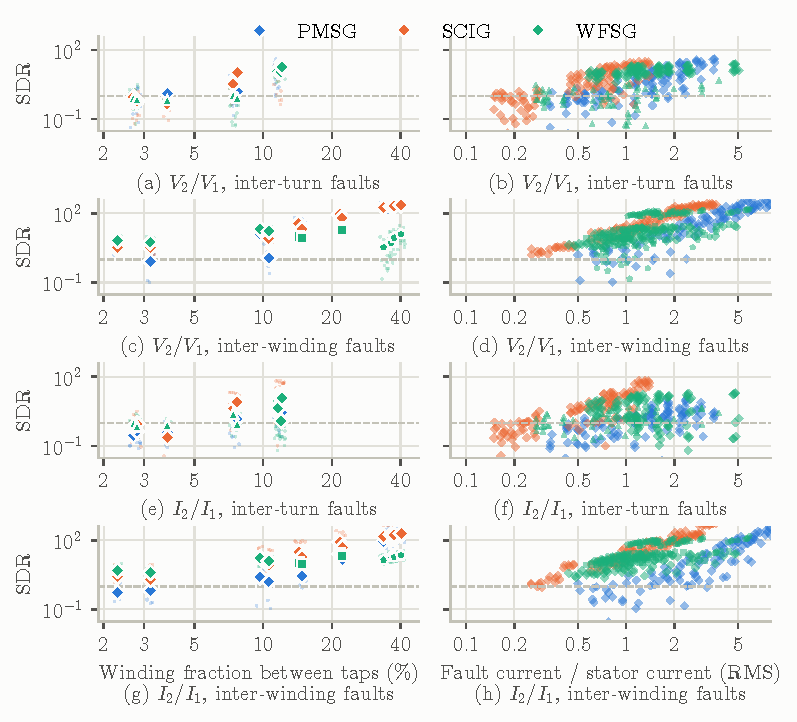
\includegraphics[width=\textwidth]{G_severity_combined}
\caption{SDR of $V_2/V_1$ (\textbf{a}--\textbf{d}) and $I_2/I_1$ (\textbf{e}--\textbf{h}) against the design-level extent (left) and the physical severity (right), three alternatives, three-cycle windows}\label{fig:severity}
\end{figure}

\subsection{Operating envelope}\label{sec:res-op}

Speed dominates the operating-point dependence: in the PMSG the median SDR of the best feature rises from 5--9 at 1200\,rpm to 16--21 at 1800\,rpm and the detectable share from 79--83 to 92--96\,\%, in the SCIG from 16--18 to 44--51 and from 92--96 to 96--100\,\%; torque changes little. Two cautions apply: the dependence is consistent with a resistor-limited fault current that scales with speed, so it is a property of the emulation as much as of the machines; and the pooled null is a mixture over operating points (the share of trials whose healthy change exceeds the pooled 95th percentile is 0--16\,\% by speed for the key features), so the 5\,\% false-alarm reading holds on average over the envelope. Both make the lowest monitored speed a parameter of the requirement.

\subsection{Observation suites and the design decision}\label{sec:res-suites}

Table~\ref{tab:suites} gives the suite results for the PMSG and SCIG at five-cycle windows, Table~\ref{tab:suites3} (Appendix~\ref{app:appendix}) for the three alternatives on the common feature set at three cycles, and Table~\ref{tab:decision} the decision table of step~5. For the PMSG, current transducers alone resolve inter-turn faults from 7.4\,\% and inter-winding faults from 9.7\,\%; three voltage transducers take these to 3.8 and 2.3\,\%, and neither controller access nor a torque transducer improves the fixed-feature result further. The drive-internal suite reaches 7.4\,\% for inter-turn faults through the duty-cycle negative sequence, a weaker version of the signature the measured terminal voltage carries. For the SCIG the cheapest suites already reach what any suite reaches---7.4\,\% for inter-turn faults through $I_2/I_1$ or, with no added sensor, the $d$-axis PI output, and 2.3\,\% for inter-winding faults---and additional hardware raises the detectable share rather than the reach. For the WFSG every suite detects all inter-winding faults from 2.3\,\% and 78--98\,\% of the inter-turn trials at the matching impedance, and the field current alone detects 86 and 100\,\%. The nested selection of the fixed feature changes no share by more than five points (Table~\ref{tab:suites3}); the oracle shares come with false-alarm rates of 44--78\,\% on the healthy trials for the large suites and are upper bounds only. A shaft torque transducer adds nothing for winding faults on the two machines on which it was available (the torque features' healthy relative change exceeds 100\,\% on the SCIG and their median SDR is below 0.3 on the PMSG).

%% BEGIN GENERATED tab_suites -- written by scripts/make_tables.py from results/tables; do not edit by hand
\begin{table}[t]
\tabsize
\setlength{\tabcolsep}{3pt}
\caption{Observation suites versus what they detect, PMSG and SCIG, five-cycle windows: best fixed feature, its MDE (\%) and detectable share (\%)}\label{tab:suites}
\begin{tabular}{@{}lllllll@{}}
\toprule
Suite & PMSG feature & MDE & DS [oracle] & SCIG feature & MDE & DS [oracle] \\
\midrule
\multicolumn{6}{@{}l}{\emph{Inter-turn faults}} \\
drive-internal & $D_2/D_1$ & 7.4 & 64 [87] & PI$_d$\,2$f_e$ & 7.4 & 78 [99] \\
3 CT & $I_2/I_1$ & 7.4 & 56 [77] & $I_2/I_1$ & 7.4 & 75 [87] \\
3 CT + 3 VT & $V_2/V_1$ & 3.8 & 76 [88] & $I_2/I_1$ & 7.4 & 75 [90] \\
3 CT + 3 VT + drive & $V_2/V_1$ & 3.8 & 76 [95] & PI$_d$\,2$f_e$ & 7.4 & 78 [99] \\
+ torque transducer & $V_2/V_1$ & 3.8 & 76 [95] & PI$_d$\,2$f_e$ & 7.4 & 78 [99] \\
\multicolumn{6}{@{}l}{\emph{Inter-winding faults}} \\
drive-internal & $D_2/D_1$ & 14.3 & 90 [100] & PI$_d$\,2$f_e$ & 2.3 & 100 [100] \\
3 CT & $I_2/I_1$ & 9.7 & 81 [94] & $I_2/I_1$ & 2.3 & 100 [100] \\
3 CT + 3 VT & $V_2/V_1$ & 2.3 & 94 [97] & $I_2/I_1$ & 2.3 & 100 [100] \\
3 CT + 3 VT + drive & $V_2/V_1$ & 2.3 & 94 [100] & PI$_d$\,2$f_e$ & 2.3 & 100 [100] \\
+ torque transducer & $V_2/V_1$ & 2.3 & 94 [100] & PI$_d$\,2$f_e$ & 2.3 & 100 [100] \\
\botrule
\end{tabular}
\footnotetext{Oracle: per-trial best feature, its detectable share in brackets (false-alarm rates in Table~\ref{tab:suites3}); features failing the reliability screen are excluded for that machine.}
\end{table}
%% END GENERATED tab_suites

The decision table turns this into the selection of step~5. At $\alpha=0.95$ no suite on any alternative meets an inter-turn requirement of 3 or 5\,\% with 95\,\% bootstrap confidence; the PMSG's voltage suite is the only candidate below 5\,\% and its verdict is uncertain, a consequence of the three-cycle windows and the coarse extent grid. At 8\,\% the drive-internal suite meets the requirement on the PMSG and the SCIG, i.e.\ no added sensor is needed for either; the WFSG's inter-turn verdicts are bounded by its smallest tested extent. For inter-winding faults the SCIG and the WFSG meet every requirement from 3\,\% with the drive-internal suite, whereas the PMSG needs current transducers at 12\,\% and is uncertain below (its five-cycle result, Table~\ref{tab:suites}, reaches 2.3\,\% with voltage transducers). Relaxing $\alpha$ to 0.90 admits the PMSG's voltage suite at 5\,\% for inter-turn faults; tightening it to 0.99 removes the PMSG's current-only option at 12\,\% for inter-winding faults.

%% BEGIN GENERATED tab_decision -- written by scripts/make_tables.py from results/tables; do not edit by hand
\begin{table}[t]
\tabsize
\setlength{\tabcolsep}{3pt}
\caption{Decision table: cheapest suite whose MDE meets $e_{\mathrm{req}}$ with probability $\ge0.95$, per alternative, fault class and $\alpha$}\label{tab:decision}
\begin{tabular}{@{}llcccccc@{}}
\toprule
\multirow{2}{*}{$\alpha$} & \multirow{2}{*}{$e_{\mathrm{req}}$ (\%)} & \multicolumn{2}{c}{PMSG} & \multicolumn{2}{c}{SCIG} & \multicolumn{2}{c}{WFSG} \\
\cmidrule(lr){3-4}\cmidrule(lr){5-6}\cmidrule(l){7-8}
 & & IT & IW & IT & IW & IT & IW \\
\midrule
0.90 & 3 & (3CT+3VT)? & (drive)? & none & drive & none & drive \\
0.90 & 5 & 3CT+3VT & (drive)? & none & drive & none & drive \\
0.90 & 8 & drive & (drive)? & drive & drive & none & drive \\
0.90 & 12 & drive & 3CT & drive & drive & drive & drive \\
0.95 & 3 & (3CT+3VT)? & (drive)? & none & drive & none & drive \\
0.95 & 5 & (drive)? & (drive)? & none & drive & none & drive \\
0.95 & 8 & drive & (drive)? & drive & drive & none & drive \\
0.95 & 12 & drive & 3CT & drive & drive & drive & drive \\
0.99 & 3 & none & none & none & drive & none & drive \\
0.99 & 5 & (3CT+3VT)? & none & none & drive & none & drive \\
0.99 & 8 & drive & none & drive & drive & none & drive \\
0.99 & 12 & drive & (drive)? & drive & drive & drive & drive \\
\botrule
\end{tabular}
\footnotetext{Three-cycle windows; probabilities from 1000 bootstrap resamples. Suites ordered drive $<$ 3CT $<$ 3CT+3VT $<$ 3CT+3VT+drv; exc: WFSG field current; IT: inter-turn; IW: inter-winding. `(suite)?': no suite meets with that confidence and the cheapest suite with an uncertain verdict is shown; `none': every suite fails. WFSG inter-turn verdicts are bounded by its smallest tested extent at the matching impedance (11.6\,\%).}
\end{table}
%% END GENERATED tab_decision

\subsection{Transfer across alternatives}\label{sec:res-transfer}

Table~\ref{tab:transfer} reports step~6 for the PMSG--SCIG pair and Table~\ref{tab:transfer3} (Appendix~\ref{app:appendix}) for the three alternatives; the figures quoted below are AUCs on the out-of-reference windows, and the values on all windows agree with them to within 0.02, so the windows used for normalisation do not drive the result. In physical units a gradient-boosted detector reaches an area under the receiver operating characteristic curve (AUC) of 0.87--0.91 within a machine on unseen tap pairs but 0.78 (PMSG$\to$SCIG) and 0.55 (SCIG$\to$PMSG) across; with its features scaled on the target machine's healthy trials, a commissioning baseline, 0.82 and 0.75, and a logistic detector under that rule falls below chance in one direction (0.45); with each feature referenced to the first half of the trial's own reference interval, 0.91 and 0.84, against 0.91--0.94 within a machine, and a logistic detector transfers at 0.89 and 0.87. The threshold that gives 1\,\% false positives on all negatives fires on 0--3\,\% of the healthy trials' fault-time windows, the only negatives that contain the contactor operation. Between the three alternatives, self-referenced detectors transfer in all six directions with AUC 0.80--0.98 on the out-of-reference windows, and a detector trained on two machines detects the faults of the third with 0.83 (PMSG), 0.88 (SCIG) and 0.97 (WFSG; optimistic, as that bench has no healthy trials). Restricted to each suite's features, every suite transfers at 0.82--0.95 when self-referenced and at 0.62--0.90 under the commissioning baseline.

%% BEGIN GENERATED tab_transfer -- written by scripts/make_tables.py from results/tables; do not edit by hand
\begin{table}[t]
\tabsize
\caption{Transfer of a window-level detector between PMSG and SCIG: AUC on all windows / AUC on the out-of-reference windows}\label{tab:transfer}
\begin{tabular}{@{}llcccc@{}}
\toprule
Referencing & Model & P$\to$P & S$\to$S & P$\to$S & S$\to$P \\
\midrule
physical units & logistic & 0.78/0.78 & 0.79/0.80 & 0.71/0.71 & 0.59/0.59 \\
physical units & GBDT & 0.88/0.87 & 0.90/0.91 & 0.78/0.78 & 0.55/0.55 \\
$z$ on target's healthy trials & logistic & 0.78/0.78 & 0.79/0.80 & 0.71/0.71 & 0.44/0.45 \\
$z$ on target's healthy trials & GBDT & 0.88/0.87 & 0.90/0.91 & 0.82/0.82 & 0.75/0.75 \\
$|z|$ vs own reference & logistic & 0.90/0.89 & 0.94/0.93 & 0.90/0.89 & 0.88/0.87 \\
$|z|$ vs own reference & GBDT & 0.92/0.91 & 0.95/0.94 & 0.92/0.91 & 0.86/0.84 \\
\botrule
\end{tabular}
\footnotetext{Out-of-reference windows: those outside the normalising set (Section~\ref{sec:computation}). P$\to$P, S$\to$S: cross-validation grouped by tap pair; P$\to$S, S$\to$P: trained on one machine, tested on the other.}
\end{table}
%% END GENERATED tab_transfer

\subsection{Robustness and the two nulls}\label{sec:res-robust}

Table~\ref{tab:sens} (Appendix~\ref{app:appendix}) shows how the tuning choices move the design quantities, with the screen applied at every setting. The inter-turn MDEs of all five key features are the same at three, five and eight cycles on both machines and the detectable shares move by at most six points; for inter-winding faults one MDE moves (the PMSG's $V_2/V_1$, 9.7\,\% at three cycles against 2.3\,\% at five and eight). Tightening the null quantile from 0.95 to 0.99 lowers the shares by 3--9 points and moves two PMSG inter-winding MDEs up one level; relaxing it to 0.90 raises the shares by up to 9 points and moves one down. No ordering of the two machines reverses, but the PMSG's inter-winding suite conclusion depends on $\alpha$ and on the window length (Table~\ref{tab:decision}). At $\alpha=0.95$ the screen removes up to three weak features per machine and window length (Appendix~\ref{app:computation}); none of the five key features is removed at any setting, and the three-cycle result of $V_2/V_1$ on the PMSG (two false alarms in nine healthy trials) passes the binomial rule. An absolute-change variant of the SDR, which removes the healthy level of the feature from numerator and null, ranks the 30 features with a Spearman correlation of 0.92--0.98 against the relative variant and picks the same three top features in every machine and class. The bootstrap intervals (Table~\ref{tab:mde}) put the median SDRs within a factor of two to four and the shares within $\pm$8--10 points.

Table~\ref{tab:between} (Appendix~\ref{app:appendix}) replaces the reference immediately before the fault by the healthy trial recorded at the same operating point at another time, a commissioning baseline: the null of the four key features widens by a factor of 1.6 to 4.9, the median SDR of the inter-turn features falls to about one (PMSG $V_2/V_1$ from 3.0 to 1.1; SCIG $I_2/I_1$ from 4.5 to 1.1) and their detectable shares to 20--59\,\%, while inter-winding faults remain detectable in 67--94\,\% of trials. The MDEs reported here are therefore statements about a short-horizon change detector; a monitor that compares against an old baseline needs the wider null.
%% ----------------------------------------------------------------------
%% discussion
%% ----------------------------------------------------------------------

\section{Discussion}\label{sec:discussion}

\subsection{What the demonstration establishes about the method}

The demonstration supports four claims about the method that do not depend on which machine came out ahead, and it corrects the naive form of two of them.

\emph{The design-level description of a failure mode does not fix its physical severity.} A short-circuit of the same winding fraction produced a fault current that differed by about 10\,\% between the PMSG and the SCIG in amperes and by a factor of 2.3 relative to the stator current the sensors see; on the WFSG bench extent and fault impedance were confounded. A method that compares alternatives on a failure-mode class must therefore carry two severity axes---the design-level one, on which requirements are written, and a physical one, on which the alternatives are compared---and state which one a number refers to; for resistor-limited emulation the physical axis is predictable at the design stage from volts per turn, speed and the resistance.

\emph{Where a failure becomes observable is a property of the machine--drive combination, and the SDR must be read with its decomposition.} In the PMSG the winding asymmetry appeared in the terminal voltage, in the SCIG in the magnetising-axis current and its controller action, in the WFSG additionally in the field current and the current harmonics; the incremental negative-sequence impedance under fault was twice as large in the PMSG drive as in the SCIG drive. The version of this claim in which ``the control structure decides'' is not supported: both machines run the same controller, and Table~\ref{tab:decomp} shows that the SCIG's higher SDR on current and $d$-axis features is entirely a quieter healthy null. The SDR is designed to credit a quiet alternative, but a design team must know whether an alternative wins by signature or by silence, because the two generalise differently: a signature is a property of the fault physics, a null of the sensing and control chain and of the operating regime, which a design-stage instantiation cannot simulate (Section~\ref{sec:design-stage}).

\emph{The cheapest adequate observation suite depends on the alternative and on the requirement, and here it would change the monitoring specification, not the architecture.} With three current transducers the PMSG reaches 7.4\,\% (inter-turn) and 9.7\,\% (inter-winding); three voltage transducers take it to 3.8 and 2.3\,\% and buy nothing on the SCIG, whose current-only or drive-internal suites already reach 7.4 and 2.3\,\%. The decision table makes the requirement explicit: around 8\,\% of a branch all three alternatives meet it with drive-internal quantities and diagnosability does not discriminate between them; below 5\,\% only the PMSG with voltage transducers is a candidate, with an uncertain verdict at the confidence demanded. The method would change an architecture decision only if, for one alternative, no affordable suite met the requirement; here it changes what is specified for each: a measured detection rating per alternative and suite, with its uncertainty, in place of an assigned one.

\emph{A monitoring design transfers across alternatives only under the right referencing rule, and the rule is a short-horizon one.} A detector built on one machine and applied to another in physical units lost much of its performance; features scaled on the target machine's healthy trials---a commissioning baseline---recovered part of it and were harmful in one direction; features referenced to the first half of each trial's own reference interval transferred in all six directions between the three machines and from any two to the third. The between-trial null (Table~\ref{tab:between}) explains why: against a baseline recorded at another time, the inter-turn signatures sit at SDR $\approx1$. For a product family the specification rule is a change detector on self-referenced deviations over a short horizon; a monitor that compares against an old baseline must be calibrated on the wider null.

\subsection{Design implications}

For the wind-turbine generator, with the scope of Section~\ref{sec:threats}: a PMSG with full-power conversion should be specified with terminal voltage measurement---or another observable of the terminal asymmetry, such as the zero-sequence voltage where a neutral is accessible \citep{Urresty2012}---if inter-turn faults below about 7\,\% of a branch are to be detected by threshold monitoring, its controller's commanded quantities carrying a weaker version of the signature. An SCIG reaches the same detectability with current transducers alone or with no added sensor, and additional hardware buys robustness rather than reach. A wound-field machine with a static exciter offers a further drive-internal channel, the field current, whose 2$f_e$ ripple detected every inter-winding fault and most inter-turn faults; a brushless exciter would not expose it \citep{Neti2009}. A shaft torque transducer, as filtered on these benches, is not worth specifying for winding faults. Two industrial parameters change these statements and are computable at the concept stage: the ratio of current-loop bandwidth to twice the electrical frequency, which for a direct-drive multi-megawatt PMSG at a fundamental near 10\,Hz will push the signature further into the controller and the voltage than in these 40--60\,Hz machines; and the grid-connected, unregulated stator of a doubly-fed generator, where the migration is absent and current-signature routes regain their reach.

\subsection{Applying the method elsewhere}

Nothing in Section~\ref{sec:method} is specific to electrical machines, but the scope conditions of Section~\ref{sec:scope} are. A gearbox family would use tooth-damage size as extent, vibration and oil-debris suites, and seeded-damage trials with a healthy run before each damage step; a battery-pack family would use cell-capacity loss, voltage, temperature and impedance suites, and trials in which a degraded cell is switched into a healthy pack.

\subsection{Threats to validity}\label{sec:threats}

The most important limitation is that each alternative is represented by one physical machine. The differences reported are differences between three machines; attributing them to topology rather than to the individual units requires replicated machines or simulated populations of each alternative under parameter variation, validated against the measured units. The demonstration is therefore regarded as establishing the method and the mechanisms, not the population-level ranking of the topologies; the two benches also differ in converter, controller, sampling rate and sensing chain.

The fault emulation is resistor-limited and the benches are laboratory scale (2--2.5\,kVA); the operating points were scaled from a 15\,MW turbine but the electrical frequency and the fault physics were not. Only winding faults and only electrical and controller observables were studied, and the suites are those the datasets can populate (Section~\ref{sec:suites}). On the WFSG the fault impedance is confounded with extent; only four tap pairs per class exist at the impedance matching the other two machines, so its inter-turn MDE is bounded, not measured; it has no healthy trials, so the reliability screen cannot be applied to it and its transfer entries lack nuisance-transient negatives; and 81 of its 438 trials hold fewer than three three-cycle windows. The PMSG/SCIG faulted interval contains about 55\,ms of healthy time before the relay picks up, which dilutes those SDRs slightly relative to the WFSG's.

Statistically, the pooled null is a mixture over operating points and holds its nominal false-alarm rate on average, not per speed; the null quantile is held fixed inside the bootstrap; the fixed feature is chosen on the trials it is evaluated on, which the nested variant shows to be immaterial here; the oracle variant is a maximum over features and its false-alarm rate is reported for that reason; the minimum detectable extent is a discrete quantity on a coarse extent grid, so the continuous SDR and its ratio are the better basis for comparing alternatives. Other nuisance transients (load steps, grid events) were not in the data. Finally, the SDR characterises a short-horizon change detector; the between-trial null shows that a monitor referenced to an old baseline faces a null 1.6 to 4.9 times wider on the key features, and every MDE in this paper should be read with that qualification.
%% ----------------------------------------------------------------------
%% conclusion
%% ----------------------------------------------------------------------

\section{Conclusions}\label{sec:conclusion}

A method has been proposed that makes the diagnosability of failure modes a criterion for choosing between architectural alternatives and, jointly, for designing the condition monitoring of the chosen architecture through the observation suite that will monitor it. Its core is a scale-free, self-calibrated statistic, the signal-to-drift ratio, from which a minimum detectable extent and a detectable share above a required extent can be computed for every combination of alternative, suite and failure-mode class, with a reliability screen, bootstrap intervals and a decision table over the required extent and the false-alarm level; a six-step procedure with default rules for its framing decisions turns these into a co-selection and a transferability specification.

Applied to three types of wind-turbine generator subjected to identical winding short-circuits on open benchmark data, the method showed that the same design-level fault is not the same physical fault across the machines; that where a fault becomes visible depends on the machine--drive combination, the detectability difference between the two machines on one bench arising from their healthy non-stationarity rather than from the signature; that the cheapest observation suite meeting a requirement depends on the alternative and on the requirement, voltage transducers lowering the permanent-magnet machine's detectable extent and adding nothing for the induction machine, while around 8\,\% of a branch all three alternatives are equally diagnosable with drive-internal quantities; and that a learned detector transfers across the three machines only when its features are referenced to each trial's own preceding healthy behaviour. The findings are robust in their orderings to the method's tuning, carry tap-pair-level uncertainty, and are limited by one physical unit per alternative, laboratory scale, resistor-limited fault emulation and a single failure-mode class.

Three extensions follow: the design-stage instantiation, in which simulated faulted trials are combined with measured healthy nulls of hardware of the same class and validated on a few physical trials, so that the method applies before hardware exists and machine-level differences become population-level statements; other failure-mode classes and observables---bearing and rotor faults with vibration and flux observables, zero-sequence and Park's-vector features for the winding faults studied here---and a mechanical or electrochemical family, to test the claim to generality; and a cost model including integration, maintenance and missed detection in place of the ordinal ranking of suites, so that the co-selection can be posed as an optimisation. The released code, which reproduces every result from the public data, is the starting point for all three.

\backmatter

\bmhead{Acknowledgements}
The author thanks the InnovaPower group of the University of S\~ao Paulo for publishing the benchmark datasets on which this work rests.

\section*{Declarations}

\bmhead{Funding}
No specific funding was received for this work.

\bmhead{Competing interests}
The author declares no competing interests.

\bmhead{Ethics approval and consent}
Not applicable.

\bmhead{Data availability}
All data are public: the PMSG, SCIG and synchronous-generator datasets of the InnovaPower MitDev-Eletrica project (\url{https://github.com/InnovaPower/MitDev-Eletrica}; Zenodo DOIs 10.5281/zenodo.15741561, 10.5281/zenodo.17161986 and 10.5281/zenodo.13685630), licensed CC BY 4.0. The derived per-trial tables are provided with the code.

\bmhead{Code availability}
The complete analysis pipeline is released under an open licence at \url{https://github.com/htcanseven/Claude} (directory \texttt{scripts/}; an archived release with a DOI will be deposited on Zenodo at acceptance) and reproduces every number in this paper from the public data.

\bmhead{Author contributions}
H.T.C. conceived the method, designed and carried out the analysis, and wrote the paper.

\bmhead{Use of generative AI}
A large language model (Claude, Anthropic) was used under the author's direction as an assistant for code development, literature retrieval, data analysis and drafting and editing of the text. The author designed the study, verified all analyses, checked every reference against its published record, and takes full responsibility for the content. No AI-generated images are used; all figures are produced by the released code from the data.

%% ----------------------------------------------------------------------
%% appendix
%% ----------------------------------------------------------------------

\begin{appendices}

\section{Feature definitions, computation details and additional tables}\label{app:appendix}

%% BEGIN GENERATED tab_suites3 -- written by scripts/make_tables.py from results/tables; do not edit by hand
\begin{table}[t]
\tabsize
\setlength{\tabcolsep}{3pt}
\caption{Observation suites for the three alternatives, three-cycle windows, common feature set, $\alpha=0.95$}\label{tab:suites3}
\begin{tabular}{@{}llllcccc@{}}
\toprule
Suite & Machine & Feature & MDE & DS & DS nested & Oracle DS & Oracle FA \\
\midrule
\multicolumn{8}{@{}l}{\emph{Inter-turn faults}} \\
drive-internal & PMSG & $D_2/D_1$ & 7.4 & 65 & 65 & 82 & 44 \\
drive-internal & SCIG & $I_d$\,2$f_e$ & 7.4 & 78 & 78 & 93 & 78 \\
drive-internal & WFSG & $I_q$\,2$f_e$ & 11.6$^{\mathrm{a}}$ & 91 & 87 & 96 & -- \\
3 CT & PMSG & $I_2/I_1$ & 7.4 & 57 & 57 & 78 & 11 \\
3 CT & SCIG & $I_2/I_1$ & 7.4 & 70 & 70 & 86 & 56 \\
3 CT & WFSG & $I_a$\,h3 & 11.6$^{\mathrm{a}}$ & 98 & 86 & 94 & -- \\
3 CT + 3 VT & PMSG & $V_2/V_1$ & 3.8 & 73 & 73 & 85 & 33 \\
3 CT + 3 VT & SCIG & $I_2/I_1$ & 7.4 & 70 & 70 & 89 & 56 \\
3 CT + 3 VT & WFSG & $V_2/V_1$ & 11.6$^{\mathrm{a}}$ & 98 & 98 & 94 & -- \\
3 CT + 3 VT + drive & PMSG & $V_2/V_1$ & 3.8 & 73 & 68 & 94 & 67 \\
3 CT + 3 VT + drive & SCIG & $I_d$\,2$f_e$ & 7.4 & 78 & 78 & 97 & 89 \\
3 CT + 3 VT + drive & WFSG & $V_2/V_1$ & 11.6$^{\mathrm{a}}$ & 98 & 98 & 98 & -- \\
excitation (field current) & WFSG & $I_f$\,2$f_e$ & 11.6$^{\mathrm{a}}$ & 86 & 86 & 74 & -- \\
\multicolumn{8}{@{}l}{\emph{Inter-winding faults}} \\
drive-internal & PMSG & $D_2/D_1$ & 14.3 & 91 & 91 & 98 & 44 \\
drive-internal & SCIG & $I_d$\,2$f_e$ & 2.3 & 100 & 100 & 100 & 78 \\
drive-internal & WFSG & $I_q$\,2$f_e$ & 2.3 & 100 & 100 & 100 & -- \\
3 CT & PMSG & $I_2/I_1$ & 9.7 & 83 & 83 & 99 & 11 \\
3 CT & SCIG & $I_2/I_1$ & 2.3 & 98 & 98 & 99 & 56 \\
3 CT & WFSG & $I_2/I_1$ & 2.3 & 100 & 100 & 100 & -- \\
3 CT + 3 VT & PMSG & $V_2/V_1$ & 9.7 & 92 & 92 & 99 & 33 \\
3 CT + 3 VT & SCIG & $I_2/I_1$ & 2.3 & 98 & 98 & 100 & 56 \\
3 CT + 3 VT & WFSG & $V_2/V_1$ & 2.3 & 100 & 100 & 100 & -- \\
3 CT + 3 VT + drive & PMSG & $V_2/V_1$ & 9.7 & 92 & 92 & 100 & 67 \\
3 CT + 3 VT + drive & SCIG & $I_d$\,2$f_e$ & 2.3 & 100 & 100 & 100 & 89 \\
3 CT + 3 VT + drive & WFSG & $I_q$\,2$f_e$ & 2.3 & 100 & 100 & 100 & -- \\
excitation (field current) & WFSG & $I_f$\,2$f_e$ & 2.3 & 100 & 100 & 100 & -- \\
\botrule
\end{tabular}
\footnotetext{Fixed feature: highest median SDR among the suite's screened features. MDE (\%) at the fault impedance matching the PMSG/SCIG protocol (WFSG: 198 trials, four tap pairs per class). DS: detectable share (\%) of the fixed feature; nested: fixed feature chosen on the other tap pairs; oracle: per-trial best feature, with its false-alarm rate on the healthy trials (FA, \%; not available for the WFSG). `--': largest tested extent not detectable.}
\footnotetext[\mathrm{a}]{The smallest inter-turn extent tested on the WFSG at that impedance is 11.6\,\%, so the value is an upper bound.}
\end{table}
%% END GENERATED tab_suites3
%% BEGIN GENERATED tab_sens -- written by scripts/make_tables.py from results/tables; do not edit by hand
\begin{table}[t]
\tabsize
\setlength{\tabcolsep}{3pt}
\caption{Sensitivity of MDE/DS to the window length (3, 5, 8 cycles at $\alpha=0.95$) and to the null quantile ($\alpha=0.90$ and $0.99$ at five cycles)}\label{tab:sens}
\begin{tabular}{@{}lllccccc@{}}
\toprule
Class & Feature & Machine & 3\,c & 5\,c & 8\,c & $\alpha$\,0.90 & $\alpha$\,0.99 \\
\midrule
IT & $V_2/V_1$ & PMSG & 3.8/73 & 3.8/76 & 3.8/73 & 3.8/80 & 3.8/69 \\
IT & $V_2/V_1$ & SCIG & 7.4/69 & 7.4/73 & 7.4/75 & 7.4/76 & 7.4/65 \\
IT & $I_2/I_1$ & PMSG & 7.4/57 & 7.4/56 & 7.4/58 & 7.4/65 & 7.4/52 \\
IT & $I_2/I_1$ & SCIG & 7.4/70 & 7.4/75 & 7.4/75 & 7.4/79 & 7.4/68 \\
IT & $I_d$\,2$f_e$ & PMSG & 12.1/29 & 12.1/30 & 12.1/28 & 12.1/33 & 12.1/24 \\
IT & $I_d$\,2$f_e$ & SCIG & 7.4/78 & 7.4/79 & 7.4/83 & 7.4/84 & 7.4/72 \\
IT & PI$_d$\,2$f_e$ & PMSG & 12.1/30 & 12.1/31 & 12.1/28 & 12.1/33 & 12.1/24 \\
IT & PI$_d$\,2$f_e$ & SCIG & 7.4/78 & 7.4/78 & 7.4/83 & 7.4/84 & 7.4/72 \\
IT & $V_q$\,2$f_e$ & PMSG & 7.4/55 & 7.4/57 & 7.4/60 & 7.4/65 & 7.7/50 \\
IT & $V_q$\,2$f_e$ & SCIG & 7.4/61 & 7.4/60 & 7.4/62 & 7.4/64 & 7.4/59 \\
IW & $V_2/V_1$ & PMSG & 9.7/92 & 2.3/94 & 2.3/94 & 2.3/94 & 9.7/91 \\
IW & $V_2/V_1$ & SCIG & 2.3/100 & 2.3/100 & 2.3/100 & 2.3/100 & 2.3/100 \\
IW & $I_2/I_1$ & PMSG & 9.7/83 & 9.7/81 & 9.7/82 & 3.2/87 & 9.7/79 \\
IW & $I_2/I_1$ & SCIG & 2.3/98 & 2.3/100 & 2.3/100 & 2.3/100 & 2.3/97 \\
IW & $I_d$\,2$f_e$ & PMSG & 21.7/71 & 21.7/72 & 21.7/69 & 21.7/74 & 21.7/69 \\
IW & $I_d$\,2$f_e$ & SCIG & 2.3/100 & 2.3/100 & 2.3/100 & 2.3/100 & 2.3/100 \\
IW & PI$_d$\,2$f_e$ & PMSG & 21.7/71 & 21.7/72 & 21.7/70 & 21.7/74 & 21.7/69 \\
IW & PI$_d$\,2$f_e$ & SCIG & 2.3/100 & 2.3/100 & 2.3/100 & 2.3/100 & 2.3/100 \\
IW & $V_q$\,2$f_e$ & PMSG & 9.7/89 & 9.7/90 & 9.7/91 & 9.7/91 & 9.7/86 \\
IW & $V_q$\,2$f_e$ & SCIG & 9.7/88 & 9.7/92 & 9.7/88 & 9.7/95 & 9.7/84 \\
\botrule
\end{tabular}
\footnotetext{Cells: MDE (\%; limit-of-detection convention; `--': largest extent not detectable) / DS (\%). IT: inter-turn; IW: inter-winding.}
\footnotetext[\mathrm{a}]{The feature fails the reliability screen at that setting.}
\end{table}
%% END GENERATED tab_sens
%% BEGIN GENERATED tab_between -- written by scripts/make_tables.py from results/tables; do not edit by hand
\begin{table}[t]
\tabsize
\setlength{\tabcolsep}{2.5pt}
\caption{Within-trial versus commissioning-baseline null, five-cycle windows, $\alpha=0.95$}\label{tab:between}
\begin{tabular}{@{}lllcccccc@{}}
\toprule
\multirow{2}{*}{Class} & \multirow{2}{*}{Feature} & \multirow{2}{*}{M.} & \multicolumn{2}{c}{$q_{95}$} & \multicolumn{2}{c}{Median SDR} & \multicolumn{2}{c}{DS} \\
\cmidrule(lr){4-5}\cmidrule(lr){6-7}\cmidrule(l){8-9}
 & & & within & baseline & within & baseline & within & baseline \\
\midrule
IT & $V_2/V_1$ & P & 0.086 & 0.315 & 2.99 & 1.05 & 76 & 50 \\
IT & $I_2/I_1$ & P & 0.162 & 0.268 & 1.47 & 0.978 & 56 & 48 \\
IT & PI$_d$\,2$f_e$ & P & 0.557 & 0.870 & 0.518 & 0.441 & 31 & 20 \\
IT & $V_q$\,2$f_e$ & P & 0.165 & 0.277 & 1.35 & 0.872 & 57 & 44 \\
IW & $V_2/V_1$ & P & 0.086 & 0.315 & 61.9 & 12.5 & 94 & 83 \\
IW & $I_2/I_1$ & P & 0.162 & 0.268 & 11.3 & 6.34 & 81 & 75 \\
IW & PI$_d$\,2$f_e$ & P & 0.557 & 0.870 & 4.21 & 2.4 & 72 & 67 \\
IW & $V_q$\,2$f_e$ & P & 0.165 & 0.277 & 22.4 & 10.7 & 90 & 81 \\
IT & $V_2/V_1$ & S & 0.033 & 0.111 & 4.17 & 1.45 & 73 & 59 \\
IT & $I_2/I_1$ & S & 0.034 & 0.130 & 4.52 & 1.15 & 75 & 54 \\
IT & PI$_d$\,2$f_e$ & S & 0.016 & 0.078 & 6.69 & 1.29 & 78 & 53 \\
IT & $V_q$\,2$f_e$ & S & 0.060 & 0.131 & 2.58 & 1.54 & 60 & 58 \\
IW & $V_2/V_1$ & S & 0.033 & 0.111 & 48.2 & 16.1 & 100 & 94 \\
IW & $I_2/I_1$ & S & 0.034 & 0.130 & 55.6 & 12.9 & 100 & 86 \\
IW & PI$_d$\,2$f_e$ & S & 0.016 & 0.078 & 74 & 16 & 100 & 88 \\
IW & $V_q$\,2$f_e$ & S & 0.060 & 0.131 & 24.8 & 11.2 & 92 & 86 \\
\botrule
\end{tabular}
\footnotetext{Four key features. Within: reference immediately before the fault; baseline: the healthy trial at the same operating point, recorded at another time. DS: detectable share (\%). IT: inter-turn; IW: inter-winding; P: PMSG; S: SCIG.}
\end{table}
%% END GENERATED tab_between
%% BEGIN GENERATED tab_transfer3 -- written by scripts/make_tables.py from results/tables; do not edit by hand
\begin{table}[t]
\tabsize
\caption{Transfer between the three alternatives with a self-referenced GBDT detector, three-cycle windows, common features}\label{tab:transfer3}
\begin{tabular}{@{}llcccc@{}}
\toprule
Trained on & Tested on & AUC all & AUC o.o.r. & TPR o.o.r. & FA healthy (\%) \\
\midrule
PMSG & PMSG & 0.86 & 0.85 & 0.62 & 3 \\
SCIG & SCIG & 0.92 & 0.91 & 0.76 & 1 \\
WFSG & WFSG & 0.97 & 0.97 & 0.93 & -- \\
PMSG & SCIG & 0.88 & 0.88 & 0.60 & 0 \\
PMSG & WFSG & 0.97 & 0.98 & 0.89 & -- \\
SCIG & PMSG & 0.81 & 0.80 & 0.35 & 0 \\
SCIG & WFSG & 0.95 & 0.96 & 0.86 & -- \\
WFSG & PMSG & 0.86 & 0.84 & 0.52 & 1 \\
WFSG & SCIG & 0.91 & 0.89 & 0.61 & 0 \\
SCIG+WFSG & PMSG & 0.84 & 0.83 & 0.41 & 0 \\
PMSG+WFSG & SCIG & 0.89 & 0.88 & 0.61 & 0 \\
PMSG+SCIG & WFSG & 0.97 & 0.97 & 0.88 & -- \\
\botrule
\end{tabular}
\footnotetext{Features $|z|$-referenced to the first half of each trial's own reference interval. AUC on all windows and on the out-of-reference (o.o.r.) windows; TPR: true-positive rate at 1\,\% false-positive rate (FPR) on the o.o.r. windows; FA: share of the healthy trials' fault-time windows above the threshold giving 1\,\% FPR on all negatives. The WFSG has no healthy trials, so its negatives are reference and recovery windows only and its rows are optimistic.}
\end{table}
%% END GENERATED tab_transfer3

This appendix defines the features (Section~\ref{app:features}), lists the computation details (Section~\ref{app:computation}) and gives the observation-suite results for the three alternatives (Table~\ref{tab:suites3}), the sensitivity of the design quantities to the window length and the null quantile (Table~\ref{tab:sens}), the commissioning-baseline null (Table~\ref{tab:between}) and the transfer results between the three alternatives (Table~\ref{tab:transfer3}).

\subsection{Feature definitions}\label{app:features}

Let $x_a, x_b, x_c$ be the sampled phase quantities of a window of $N$ samples at sampling frequency $f_s$, $w$ the Hann window and $f_e$ the electrical frequency of the window, estimated from the slope of the unwrapped phase of the current space vector $\tfrac{2}{3}(i_a + \mathbf{a}\, i_b + \mathbf{a}^2 i_c)$, $\mathbf{a}=e^{j2\pi/3}$, whose sign gives the phase rotation (outside 0.5--1.5 times the nominal value the nominal value is used). The complex fundamental amplitude of a signal $x$ at frequency $f$ is $X(f) = \frac{2}{\sum_n w_n}\sum_{n=0}^{N-1} x_n\, w_n\, e^{-j2\pi f n/f_s}$. Sequence magnitudes are $|X_+| = |X_a + \mathbf{a}X_b + \mathbf{a}^2X_c|/3$ and $|X_-| = |X_a + \mathbf{a}^2X_b + \mathbf{a}X_c|/3$ for an $abc$ rotation (interchanged for $acb$), evaluated at $f=f_e$ for currents ($I_1, I_2$), terminal voltages ($V_1, V_2$) and mean-removed duty cycles ($D_1, D_2$); $|X(f)|$ is a peak amplitude and is divided by $\sqrt2$ wherever it is compared with an RMS value. The RMS unbalance is $\max_k |I_{\mathrm{rms},k} - \bar I_{\mathrm{rms}}| / \bar I_{\mathrm{rms}}$ over the three phases; the harmonic ratios are $|I_a(kf_e)|/|I_a(f_e)|$ for $k=3,5,7$ and the THD is $\sqrt{\sum_{k=2}^{20}|I_a(kf_e)|^2}/|I_a(f_e)|$. For the synchronous-frame currents $i_d, i_q$ and the torques the features are the standard deviation of the mean-removed signal and its amplitudes $|Y(f_e)|$ and $|Y(2f_e)|$; for the PI outputs the standard deviation and $|Y(2f_e)|$; for the measured and commanded synchronous-frame voltages $|Y(2f_e)|$; for the field current the standard deviation and $|Y(2f_e)|$; speed and DC-link features are standard deviations. Windows are $n_c$ electrical cycles long with a hop of one cycle, and a feature is undefined for a trial whose faulted interval holds no complete window. On the WFSG bench the measured converter-side phase voltages serve as terminal voltages, the synchronous-frame voltages are obtained from them with the encoder angle, the commanded voltages are the controller's, and the electrical torque is computed from power and speed.

\subsection{Computation details}\label{app:computation}

\emph{Intervals.} PMSG and SCIG: reference interval 0.30--0.98\,s after the start of each record, split at 0.62\,s into $R_1$ (0.32\,s) and $R_2$ (0.36\,s); contactor commanded at 1.000\,s; faulted interval from 30\,ms after the command to 10\,ms before its release; the relay picks up 85--90\,ms after the command, so the faulted interval holds about 55\,ms of healthy time (at most 15\,\% of its length), which dilutes the fault-interval mean and makes the PMSG/SCIG SDRs slightly conservative; recovery windows start 0.30\,s after the release. WFSG: fault interval located from the measured fault current as the first contiguous interval in which its 10\,ms RMS exceeds $\max(0.3\,\mathrm{A}, 6\sigma)$, $\sigma$ being the standard deviation of that RMS over 0.05--0.40\,s, ending at the first fall below the threshold after 50\,ms; reference interval from 0.05\,s after the start of the record to 10\,ms before the onset, split at 0.30\,s; recovery windows start 0.15\,s after the end of the fault interval. At 23.9--63.7\,Hz a WFSG faulted interval holds between zero and eleven three-cycle windows; four trials hold none and are dropped, and 81 of 438 hold fewer than three (all 50 trials at 1671\,rpm, 26 of 206 at 1800\,rpm, 4 at 716 and 1 at 955\,rpm).

\emph{Null and screen.} The null is pooled over all 225 records of each of the PMSG and SCIG and over the 438 inter-turn and inter-winding records of the WFSG. The screen flags a feature when its count of false alarms on the nine healthy trials is incompatible with the nominal rate $1-\alpha$ at the 5\,\% level (one-sided binomial test: three or more at $\alpha=0.95$, two or more at $\alpha=0.99$, four or more at $\alpha=0.90$) and excludes features whose null quantile exceeds one. At $\alpha=0.95$ it removes, at three cycles, $D_2/D_1$ on the SCIG; at five cycles $I_d$\,1$f_e$ and speed std on the PMSG and $I_a$\,h7 and $D_2/D_1$ on the SCIG; at eight cycles PI$_d$\,std and speed std on the PMSG and $I_q$\,2$f_e$, $D_2/D_1$ and $V_{dc}$\,std on the SCIG.

\emph{Bootstrap.} 2000 resamples, seed 1. Median SDR and detectable share of a class: cluster bootstrap over the twelve tap pairs, the same resampled pairs for both machines; Wilson 95\,\% intervals for shares. Minimum detectable extent: operating-point trials resampled within each extent level and the limit-of-detection rule applied to each resample. The null quantile is held at its full-sample value. Decision table: 1000 resamples per suite, alternative, class and $\alpha$ (seed 7); a suite \emph{meets} $e_{\mathrm{req}}$ when the resample probability of $\mathrm{MDE}\le e_{\mathrm{req}}$ is at least 0.95 and \emph{fails} when it is at most 0.05.

\emph{Transfer.} Models: scikit-learn histogram gradient boosting (maximum depth 3, 200 iterations, learning rate 0.08, random state 0) and logistic regression with standardisation ($C=1$, 3000 iterations); five-fold GroupKFold with one group per tap pair and machine, healthy trials grouped by speed. The self-referencing rule uses the windows starting before 0.62\,s (PMSG/SCIG) or 0.30\,s (WFSG) as the normalising set. Metrics: area under the receiver operating characteristic curve (AUC) and true-positive rate at 1\,\% false-positive rate, on all windows and on the windows outside the normalising set, and the false-alarm rate of the all-negatives 1\,\% threshold on the fault-time windows of the healthy trials.

\end{appendices}

{\makeatletter\def\bibfont{\reset@font\fontfamily{\rmdefault}\footnotesize\selectfont}\makeatother
\setlength{\bibsep}{0.05em}
\bibliography{refs}}

\end{document}
